\chapter{EVDT Framework} \label{ch:evdt}

\section{\hlc[green]{Chapter Purpose \& Structure}}

The aim of this chapter is to detail a framework for developing a \acf{dss} for a sustainable development application, as is called for by Research Deliverable 1b:

\blockquote{\textit{A proposed framework for applying systems engineering for sustainable development in an participatory and social-justice-oriented manner.}} 

This framework, called the \acf{evdt} Framework, is intended to satisfy the need for a framework for collaboratively developing a systems-architecture-informed, multidisciplinary \ac{gis} \ac{dss} for sustainable development applications that makes significant use of remote observation data. Compared to most frameworks for applying \acf{eo} data for sustainable development, the \ac{evdt} Framework aims to to create management approaches and toolsets for sustainable development application that the stakeholders find useful; to be applicable to a wider range of spatial and temporal scales than is common in \ac{eo} applications (particularly on the smaller and shorter end of things); to involve a wider range of stakeholders throughout the development process; and to be attentive to both environmental and human wellness, rather than just one or the other. 

This chapter starts with Section \ref{sec:need}, which builds upon the lessons and priorities identified in Chapter \ref{ch:theory} in order to establish that such a need exists. Section \ref{sec:gap} then considers the extent to which various past and present approaches already satisfy this need in order to justify the creation of a new framework. That new framework is detailed in Section \ref{sec:intended}, which walks through the \ac{evdt} Framework element by element. Section \ref{sec:intended} then presents the intended uses of the framework in more detail. These sections will thus collectively propose an answer to Research Question 1: 

\blockquote{\textit{What aspects of systems architecture (and systems engineering in general) are relevant and useful for approaching issues of sustainability in complex \acf{sets}? In particular, how can they be adapted using techniques from collaborative planning theory and other critical approaches to avoid the technocratic excesses of the past?}}

The chapter concludes with Section \ref{sec:evdt-conclusion}. There I will recap the framework and set the stage for the subsequent two chapters, which present applied case studies of the \ac{evdt} Framework for those interested in concrete demonstrations. Chapter \ref{ch:conclusion} will finally revisit the \ac{evdt} Framework in light of the two case studies and discuss plans for the future. 

\section{\hlc[cyan]{The Need for a Framework}} \label{sec:need}

Before presenting the \ac{evdt} Framework, it is important to establish what motivated the creation of the framework, what the current landscape of approaches looks like, and whether any gap actually exists. This section focuses on the first of these. This motivation is heavily grounded in the lessons from Chapter \ref{ch:theory}. That chapter surveyed the fields of sustainable development, systems engineering, earth observation, \ac{gis}, participatory planning, and decision support. It considered the history and trajectory of these fields, how they overlap and intersect, and both the potential benefits and harms that they can cause. This resulted in several particular conclusions that are important for the \ac{evdt} Framework:

\begin{itemize}[itemsep=0pt,parsep=0pt]
	\item{\textbf{It is both important and urgent that we, as a society, pursue sustainable development.} As discussed in Section \ref{sec:sustainable_development}, we face various forms of resource depletion, environmental collapse, and climate change that risk significantly increasing the already unconscionable lack of access to income, health, education and more around the world.}
	\item{\textbf{Any approach to sustainable development must take a multidisciplinary approach involving the environment, societal impact, human decision-making, and technology.} As discussed in Section \ref{sec:sustainable_development}, our concepts of development and human wellness have expanded. They are no longer measured in short-term, purely individual economic / civil rights terms. We are also concerned with questions of equity, of ecosystem services, of community resilience. This broader conception of development as well as the more complicated, interconnected nature of contemporary society means that we must increasingly rely upon models and simulations to better understand the consequences of proposed policies and decisions. We increasingly understand - and appreciate - the complex relationships between these domains, relationships that were previously ignored in analyses \cite{gaheganMultivariateGeovisualization2007}. }
	\item{\textbf{The fields of systems engineering, remote observation, and \ac{gis}  have powerful tools for advancing sustainable development.}  Remote observation (Section \ref{sec:remote}) provides data that is new in kind, scale (both spatial and temporal). While it has a well developed history of monitoring environmental phenomena at the global scale, it has a much more limited use in local, human-centric applications and there is thus much potential there. Systems engineering (Section \ref{sec:se}) and \ac{gis} (Section \ref{sec:gis}) represent two approaches for corralling remote observation data along with that of many other sources for use in sustainable development. These two fields have been closely linked since their inception in the mid-20th century and both are based on the idea of using data and models to inform and support decision-making. }
	\item{\textbf{In order to avoid the technocratic harms of the past, it is important to take a participative, local community approach and focus on decision support, rather than prescriptive solutions.} Often no single, objectives solution exists for a sustainable development problem and, even if it did, our data collection and analysis methods are insufficient to reach it. In absence of such a single solution, consider and selecting a course of action must be made by the community. Such a process helps too with acceptance and implementation of the decision. A wide set of stakeholders also commonly means both a wide concept of human wellness and one that is relevant to the community in questions. This means that the primary role of systems engineering and \ac{gis} in such situations is to support decisions rather than to make them, to help communities envision potential future scenarios rather than to dictate one to them.}
\end{itemize}

These lessons establish that there are both push and pull factors motivating the creation and use of a framework for collaboratively developing a systems-architecture-informed, multidisciplinary \ac{gis} \ac{dss} for sustainable development applications that makes significant use of remote observation data. This leads to the question, do any such approaches or frameworks already exist? And to what extent do they satisfy this need?

\section{\hlc[cyan]{Identifying the Gap}} \label{sec:gap}

Now that the motivation for \textit{a} framework has been made clear, what are the already available approaches for satisfying that need? This section considers this question and seeks to identify what, if any, gap remains.

First, it is obvious that I am not the first to suggest that sustainable development is an important and urgent issue (see all of Section \ref{sec:sustainable_development}). Advocating for the use of models is not new either. Computational models have long been closely linked to the pursuit of sustainable development and with its definition, stemming from the World3 system dynamics model underlying the Club of Rome's \textit{The Limits to Growth} report in 1972 \cite{meadowsLimitsGrowth1972}. As was discussed in Section \ref{sec:se}, the development field would largely come to repudiate such efforts in the mid-to-late 1970s, only to come back around to modeling on their own terms in the subsequent decades. Thus there is nothing new in saying that modeling plays an important role in sustainable development.

But what about multidisciplinary model? There have been numerous attempts to advance the concept of multidisciplinary, integrated models in development applications. To refer to just a handful of examples:

\begin{itemize} \setlength{\itemsep}{0pt} \setlength{\parskip}{0pt}
	\item{The open source UrbanSim combines land use, transportation, and certain environmental factors in a dynamic, area-based simulation system that, similar to \ac{evdt}, is a collection of multiple models \cite{waddellUrbanSimModelingUrban2002}.}
	\item{The agent-based \ac{ilute} model simulated the urban spatial form, demographics, travel behavior, and environmental impacts for the Toronto area \cite{millerHistoricalValidationIntegrated2011}.}
	\item{The TripEnergy model combines an environmental submodel (transportation systems) and societal impact submodel (energy consumption and emissions of vehicles) \cite{needellEfficientlySimulatingPersonal2018}. It is then combined with a model of human decision-making to create Tripod, "a smartphone-based system to influence individual real-time travel decisions by offering information and incentives to optimize system-wide energy performance" \cite{azevedoTripodSustainableTravel2018}.}
	\item{Lauf et al. combined cellular automata with systems dynamics to capture both spatial dynamics and macroscale demand-supply dynamics in order to simulate residential development \cite{laufUncoveringLanduseDynamics2012}.}
	\item{Pert et al. combined environmental and decision-making in a participatory model to improve conservation outcomes \cite{pertParticipatoryDevelopmentNew2013}.}
	\item{Shahumyan and Moeckel linked together existing models in a loose manner using ArcGIS Model Builder to study transportation, mobile emissions, building emissions, and \ac{lclu} \cite{shahumyanIntegrationLandUse2017}.}
\end{itemize} 

In the field of earth science, integrated models have also become increasingly common. Originally developed for operational weather forecasting, \acp{osse} have found widespread use for designing earth observation systems at \ac{nasa} and elsewhere \cite{masutaniObservingSystemSimulation2010}, by linking models of environmental phenomena with simulations of observing platforms (both hypothetical and real). These models are rigorously validated \cite{erricoDevelopmentValidationObservingsystem2013} and are often custom-made for a particular mission. Significant progress has been made however by the Hydrological Sciences Laboratory and Earth Science Technology Office at \ac{nasa} in developing the \ac{lis}, a more reusable and inter-operable modeling tool with numerous earth sciences applications (soil moisture, hydrology, meteorology, etc.) \cite{kumarMissionSimulationEvaluation2015}. One of these uses is the easier development of \acp{osse}, as a means of facilitating technological development. Since the development of the \ac{lis}, the Hydrological Sciences Laboratory has worked to make the earth science models more accurate, utilize  a broader range of computational methods, and standardize the validation and evaluation processes for \acp{osse}.

While most of these only deal with some subset of the environment, societal impact, human decision-making, and technology, they clearly establish that there is interest and active work ongoing in multidisciplinary models. Of all of them, Shahumyan and Moeckel come the closest to addressing the need. They linked together models covering each of the four domains and even included some limited feedbacks between them \cite{shahumyanIntegrationLandUse2017}. However, they lack both an explicit inclusion of systems engineering and a participative aspect, instead relying upon proprietary, closed source code. They also do not provide a generalized framework for applying their approach to other, potentially dissimilar situations.

There are distinct advantages to the development and codification of such a concrete framework for such integrated modeling projects for sustainable development applications. Many of the above examples of integrated models were developed either without such a framework at all (a one off model intended to solve a particular problem or demonstrate a particular technique) or for a different class of applications (the \ac{osse} framework is fundamentally about designing better \acp{eos} for scientific purposes). 

So what dedicated frameworks exist that are focused more directly on sustainable development? First, there are a set intended for use by large governmental (often multi-nation and/or multi-agency) teams and that aim at national or even multinational applications. These include \ac{servir}, \ac{fews}, and various \ac{un}-affiliated programs such as the World Food Program). Even to the extent that these fully embrace multidisciplinary modeling (and they often do not), there is a real need for a framework that is dedicated for sustainable development applications of small scales, accessible to relatively small teams for specific, targeted projects.

There are some frameworks operating in this space, some of which include both systems engineering and a participative element. In 2020, Honoré-Livermore et al. sought to address the \acp{sdg} in arctic coastal regions via an approach grounded in \ac{ses} and the \ac{spade} methodology \cite{honore-livermoreAddressingSustainableDevelopment2020}. The \ac{spade} methodology was developed specifically for sustainable development applications. The five components of its name constitute five non-linear steps, each of which has various specific associated methodologies \cite{haskinsSystemsEngineeringAnalyzed2008}, as shown in Figure 3.

\begin{figure}[!htb]
\centering
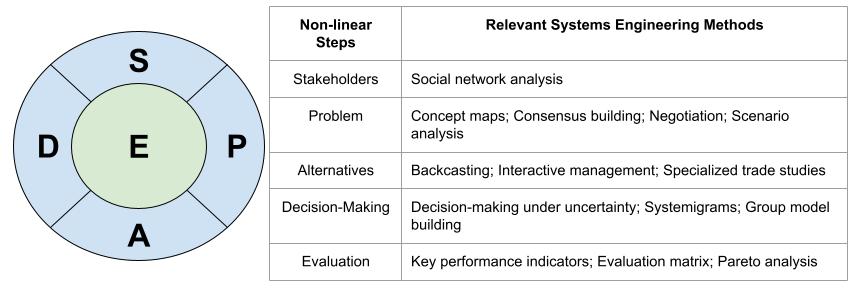
\includegraphics[scale=0.4]{Figures/chap3/spade.png}
\caption[The SPADE Methodology and associated methods]{The Stakeholders-Problem-Alternatives-Decision-Making-Evaluation (SPADE) Methodology and associated methods. Adapted from Haskins, 2008 \cite{haskinsSystemsEngineeringAnalyzed2008} as seen in \cite{reidSystemsEngineeringAppliedPendingPublication}.}
\label{fig:spade}
\end{figure}

Van Zyl and Root meanwhile used a transdisciplinary approach involving Wilbur's integral systems theory \cite{esbjorn-hargensOverviewIntegralTheory2010} and the \ac{catwoe} framework from \ac{ssm} \cite{checklandSoftSystemsMethodology2000} to design sustainable agricultural principles in New Zealand \cite{vanzylTransdisciplinaryDesignImplementation2020}.

Other recent approaches focus on scenario planning and education for understanding evolution of the urban form \cite{geyerSystemsEngineeringMethodology2014}, sustainable land-use planning that relies upon multilevel stakeholder partnerships \cite{puchol-salortUrbanPlanningSustainability2021}, a synthesis of participatory planning with systems engineering for sustainable regional planning \cite{aspenDevelopingParticipatoryPlanning2021}, and leveraging human-centered design to address the \acp{sdg} \cite{muellerUsingHumanCenteredDesign2020}. A survey of sustainable development applications of systems engineering can be found in Yang and Cormican, 2021 \cite{yangCrossoversConnectivitySystems2021}, which itself was published in a special issue of \textit{Sustainability} dedicated to systems engineering \cite{haskinsSystemsEngineeringSustainable2021}.

Common across all of these methods are a significant consideration of a wide set of stakeholders and an adoption of different systems engineering techniques for integrating these stakeholder needs into the system design and development process. They largely lack the multidisciplinary modeling component, however, and any concrete use of \ac{eo} data.

All of this clearly demonstrates that I am far from the first to argue that such multidisciplinary integration is necessary, for the potential utility for systems engineering in sustainable development, or for the use of participatory design and decision-making. I am also not the first to recognize that these all are easier said than done \cite{shahumyanIntegrationLandUse2017}. A gap remains however. There is still a need for a generalized framework that puts all of these together. We have multidisciplinary, participatory sustainable development modeling projects that lack a generalized framework. We have frameworks that individually focus on sustainable development, multidisciplinary modeling, participation on a local scale, and remote observation, but not one includes all these aspects. It is this gap that the \ac{evdt} Framework, laid out in the following section, seeks to fill.

\section{\hlc[cyan]{The Framework}} \label{sec:framework}

The \ac{evdt} Framework is process for developing a \ac{dss} for a sustainable development application. This process is characterized by five basic elements, shown in Figure \ref{fig:evdt_framework} and enumerated as: 

\begin{enumerate}[label=\emph{\Alph*)},itemsep=0pt,parsep=0pt]
	\item{The use of systems architecture \& stakeholder analysis to identify needs, design the \ac{dss}, and understand the context through the use of the \acf{saf}. This requires significant engagement with as many of the stakeholders as is feasible (if not more). Usually two or more iterations through the \ac{saf} cycle are required.}
	\item{A concept of the sustainable development application as a complex \ac{sets}, typically involving the Environment, Human Vulnerability and Societal Impact, Human Behavior and Decision-Making, and Technology Design. This concept undergirds the \ac{dss} architecture and is critical as it provides the capability both for detailed technical analysis as well as feeding back into the design of data collection systems. \label{item:evdt}}
	\item{An interactive \ac{dss}. This can take the form of an in-browser page, a standalone application for a computer or phone, or even a tabletop exercise with paper documents.}
	\item{A consideration towards modularity and re-use in future applications. This includes both technical components of the \ac{dss} product and broader capacity building in the community.}
	\item{Collaborative development of the \ac{dss} that continues beyond initial stakeholder engagement.}
\end{enumerate}

Each of these elements span the entire lifecycle of an \ac{evdt} project, but can still be usefully considered in the order listed. The following subsections walk through each of these elements. A later section in this chapter address in more detail the intended uses and users of the framework.

\begin{landscape}
\begin{figure}[t]
	\centering
	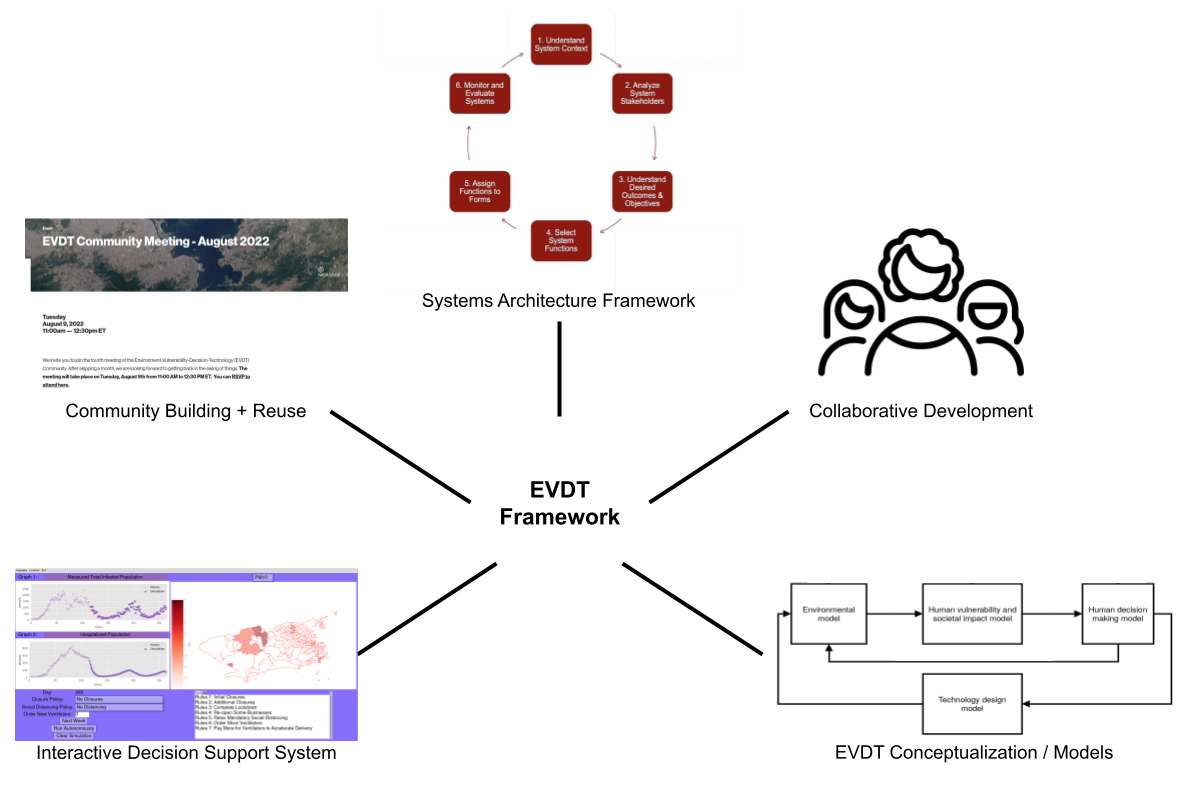
\includegraphics[scale=0.225]{Figures/chap3/evdt_framework.png}
	\caption[Overall EVDT Framework]{Overall EVDT Framework. Lettered circles label the components of the framework. A) The iterations of the Systems Architecture Framework; B) Collaborative development; C) the environment-vulnerability-decisionmaking-technology conceptualization; D) the interactive decision support system output; E) Modularity and re-use}
	\label{fig:evdt_framework}
\end{figure}
\end{landscape}

%%%%%%%%%%%%%%%%%%%%%%%%%%

%Yamu et al. argue that urban modeling should treat the urban form as a \ac{cas} and use fractal metrics to develop scenarios for planning purposes \cite{yamuAssumingItAll2016}.

\subsection{\hlc[cyan]{Initiating an EVDT Project}} \label{sec:initiate}

Much of the following sections detail how the \ac{evdt} Framework refines a motivating question, understands its context, and determines an approach for answering it. Prior to all of this though is how one realizes there is a question to be asked and that the \ac{evdt} Framework is the right approach for addressing it. Here I seek to briefly provide an answer.

Any \ac{evdt} project must start with a local stakeholder with a sustainable development problem to solve. This stakeholder, who we refer to as a Local Context Expert (See Section \ref{sec:intended} for more discussion on this designation), must also be willing to dedicate the time and effort to either lead the \ac{evdt} project or heavily collaborate with outside facilitators (such as the Space Enabled Research Group that I am a part of). Maybe the head of a local company wants help dealing with an invasive plant species \cite{ovienmhadaInclusiveDesignEarth2021}. Or officials in a municipal planning agency want assistance with improving coastal resiliency \cite{lombardoEnvironmentVulnerabilityDecisionTechnologyFrameworkDecision2022}.   Or a tribal self-governance director wants support in planning natural resource management \cite{lombardoUtilizingSatelliteEarth2022}.

In our experience, this initiating Local Context Expert is usually the one who first identifies the problem and pitches the collaboration, with the external facilitator proposing the \ac{evdt} Framework as a potential approach. The \ac{evdt} Framework does not rule out the idea of an external facilitator identifying a problem and initiating conversation, but caution should be taken in such circumstances to avoid thrusting a malformed question upon a community.

The initiating Local Context Expert should not be assumed to be the sole representative of their community nor should their problem formulation be accepted as written in stone. Much of Section \ref{sec:saf} details how additional stakeholder perspectives are considered and how the motivating question can be refined. As a participative methodology focused on decision-support, the \ac{evdt} Framework requires some level of participation from a variety of stakeholders. If not even a single person can be found to be an initial Local Context Expert, or that person is reluctant to participate, this is likely be a sign that this venue is not right for an \ac{evdt} project at this time.

Beyond these conditions, there are not any particular restrictions on the kind of problem that the \ac{evdt} Framework can be used for. While one of the motivations for its creation was to be able to handle applications at relatively small spatial scales (neighborhoods, small towns, municipalities), the framework is not restricted to such applications. Similarly, while the case studies presented in this thesis focus on informing policy decisions, there are other potential applications of the \ac{evdt} Framework (See Section \ref{sec:intended} for discussion of such uses). 

So, with at least one Local Context Expert, at least one \ac{evdt} facilitator, and a (perhaps vague) initial sustainable development question, we are ready to move onto the first full element of the \ac{evdt} Framework: the \ac{saf}.


\subsection{\hlc[cyan]{A: System Architecture Framework}} \label{sec:saf}

The \acf{saf} is the first element of the \ac{evdt} Framework. It is used to learn about the system in question, solicit stakeholder perspectives, and identify the necessary features of the \ac{dss} to be developed later on. This section will provide an overview of the \ac{saf} and its history. The following subsections will then go through each step and then explain why two iterations of the \ac{saf} are shown in Figure \ref{fig:evdt_framework}.

The \ac{saf} as seen in this thesis was developed by Danielle Wood and has gone through several revisions and expansions since its inception \cite{woodAnalysisTechnologyTransfer2013, woodApplyingSystemsArchitecture2014, kazanskyCurrentPotentialRole2016}. It predates the creation of the \ac{evdt} Framework. The version here is based on the most recent version, as seen in Ovienmhada et al. \cite{ovienmhadaInclusiveDesignEarth2021}. The \ac{saf} itself builds upon prior work in systems engineering, particularly the subdiscipline of systems architecture as laid out by Maier, Rechtin, Crawley, Cameron, and Selva \cite{crawley2004, crawleySystemArchitectureStrategy2015, maierArtSystemsArchitecting2009}, with \ac{saf} drawing its definitions most directly from Crawley et al. \cite{crawley2004}. This prior work tended to be nominally application agnostic, but in practice tended to see application in large aerospace and civil engineering projects. \ac{saf} is similarly application agnostic but has seen its primary uses in international collaborations \cite{pfotenhauerArchitectingComplexInternational2016} and sustainable development \cite{ovienmhadaInclusiveDesignEarth2021}. 

It should be noted that the \ac{saf} includes a variety of technical terms that have similar but not identical definitions to their colloquial use. This terms will typically be indicated with capitalization (e.g. System Boundary). Definitions will be supplied at their first occurrence, but are also listed in the glossary found in Appendix \ref{glossary}.

As defined by Maier, \textit{systems architecture} the art and science of creating and building complex systems, and in particular that part of systems development most concerned with scoping, structuring, and certification \cite{maierArtSystemsArchitecting2009}. This tends to refer to the high level form and function of a system, rather than detailed design. Others, such as Crawley prefer to characterize systems architecture as the mapping of Function to Form such that the essential features of the system are represented. System Functions here mean the specific actions or processes that the system performs. System Forms meanwhile refers to the approaches and structures used to enable the Functions (i.e. the ``stuff" of the system, including tangible objects, software-based objects and organizations). The intent of architecture is to reduce ambiguity, employ creativity, and manage complexity \cite{crawleySystemArchitectureStrategy2015}. Arguably this is a more specific formulation of Maier's definition. In general, Space Enabled and I tend to use Crawley's definition, both due to its clarity, and for the various qualitative and quantitative methods that have been developed to work well with this formulation. 

The current version of \ac{saf} involves six steps, shown in Figure \ref{fig:saf}. It seeks to center the full network of stakeholders and invite them into a collaborative development process. This process can be used to describe an existing system, identify some system modification, or design an entirely new system. By stakeholders, I mean the people, organizations, and communities that either influence the design and operation of the system or are impacted by the system, or as NASA defines the term: those who are affected by or accountable for an undertaking \cite{nasaofficeofthechiefengineerNASASystemsEngineering2004}. 

\begin{figure}[!htb] 
\centering
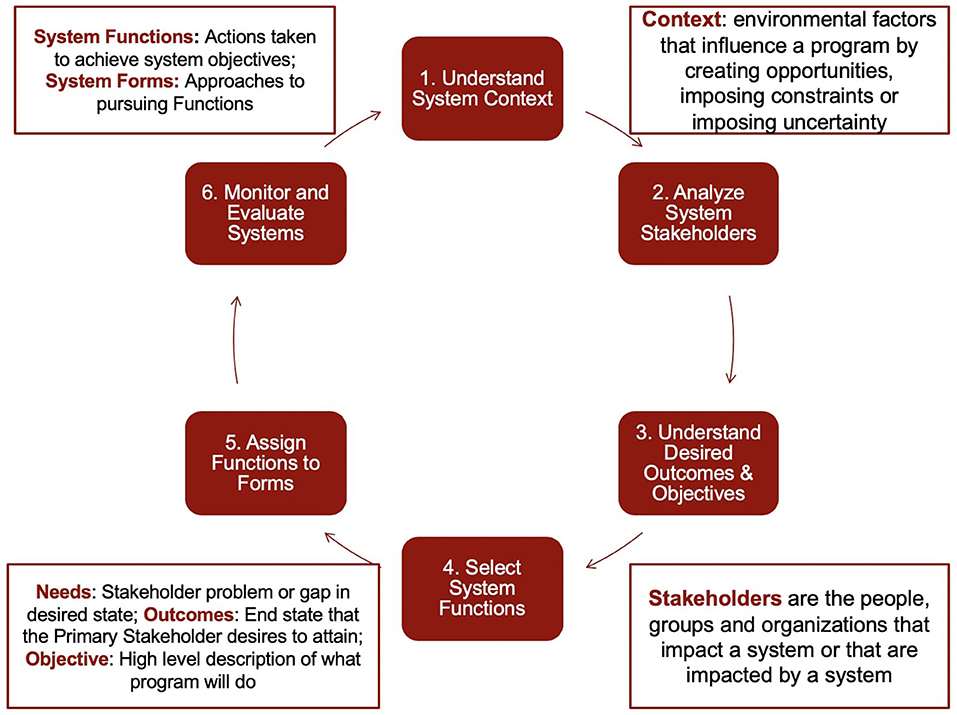
\includegraphics[width=0.9\textwidth]{Figures/chap3/SAF.jpg}
\caption[Six steps of SAF]{Six steps of \ac{saf}.}
\label{fig:saf}
\end{figure}

The primary benefit of a systems architecture approach such as \ac{saf} is, as Crawley articulates
\cite{crawley2004}:

\begin{enumerate}[itemsep=0pt,parsep=0pt]
	\item{Architecture is a way to understand complex systems.}
	\item{Architecture is a way to design complex systems}
	\item{Architecture is a way to design standards and protocols to guide the evolution of long-lived systems.}
	\item{Architecture is a way to manage complex systems.}
\end{enumerate}

As discussed in Sections \ref{sec:se} and \ref{sec:se_critique}, traditionally systems engineering focused on a single stakeholder: the client, with the benefits accruing to that stakeholder primarily. More recent approaches, such as \ac{saf}, expand this to considering the perspectives of multiple stakeholders, though still primarily only using stakeholder input to inform system requirements the beginning of the development cycle. Even \ac{saf} though only explicitly requires the involvement of a wide set of stakeholders during Steps 1-3. If we desire the benefits of a system to not just accrue to central authorities or technocrats but rather to be held by the community themselves, we must ensure keep stakeholders involved through the full cycle.

The following subsections walk through the \ac{saf} steps individually, providing potential methods to achieve each step and discussing continued stakeholder involvement. Section \ref{sec:evdt-collab} will expand how to ensure collaboration and participation throughout the process as well.

A summary of useful methods for each step of \ac{saf} is available in Table \ref{tab:saf_methods}, along with useful references. Italicized methods are defined in the corresponding following subsection of this chapter. It should be noted that many of these methods are useful in multiple steps but are listed here in the step that they are primarily associated with. Not all methods are recommended for every application. 

\begin{table}[!htb]
\caption[Methods for SAF Steps]{Methods for SAF steps. Italicized methods are defined in the corresponding following subsection of this chapter.}
\label{tab:saf_methods}
\begin{center}
\scriptsize
\begin{tabular}{ C{2.5cm} |  L{5.75cm}  L{5.75cm} } \hline

\textbf{SAF Step} & \multicolumn{2}{c}{\textbf{Useful Methods}}  \\ \hlinewd{2pt}

\multirow{7}{2.5cm}{\centering \textbf{1.} Understand System Context} & \multicolumn{1}{c}{Data Collection} & \multicolumn{1}{c}{Analysis/Synthesis} \\
& - Academic literature survey & - Critical Analysis\\
& - Survey of newspapers, periodicals, popular media, and local museums & - \textit{System Scales/Dimensions} \\ 
& - Informal conversations with stakeholders & - History Narrative\\
& - Stakeholder interviews & \\
& - Stakeholder surveys & \\
& - Direct observation & \\ \hline

\multirow{4}{2.5cm}{\centering \textbf{2.} Analyze System Stakeholders} & \multicolumn{2}{l}{- \textit{Primary-Secondary-Tertiary Classification}} \\
& \multicolumn{2}{l}{- Flowchart relational mapping \cite{jaffeEnvironmentalEconomicSystems2022}} \\
& \multicolumn{2}{l}{- Stakeholder Value Network Analysis \cite{fengDependencyStructureMatrix2010a}} \\
& \multicolumn{2}{l}{- Agent-based modeling \cite{battyCitiesComplexity2005}} \\ \hline

\multirow{3}{2.5cm}{\centering \textbf{3.} Understand Desired Outcomes \& Objectives} & \multicolumn{2}{l}{- Unified objective function and constraints \cite{hazelriggFundamentalsDecisionMaking2012}} \\
& \multicolumn{2}{l}{- Monetary conversions (e.g. ecosystem services) \cite{grootEcosystemServicesValuation2020, viscusiEconomicsRegulationAntitrust2018, ackermanPricingPricelessCostBenefit2001}} \\
& \multicolumn{2}{l}{- Multi-stakeholder negotiations \cite{fitzgeraldRecommendationsFramingMultistakeholder2016}}\\ \hline

\multirow{3}{2.5cm}{\centering \textbf{4.} Select System Functions \& Objectives} & \multicolumn{2}{l}{- Multicriteria negotiations \cite{sparrevikUseMulticriteriaInvolvement2011}} \\
& \multicolumn{2}{l}{- Pairwise comparisons \cite{motieyanSustainableUrbanPlanning2017}} \\
& \multicolumn{2}{l}{- Delphi method  \cite{morganUrbanPlanningUsing1979}} \\ \hline

\multirow{4}{2.5cm}{\centering \textbf{5.} Assign Functions to Forms}
& \multicolumn{2}{l}{- \textit{System diagramming}} \\
& \multicolumn{2}{l}{- Scenario planning workshops \cite{goodspeedScenarioPlanningCities2020}} \\
& \multicolumn{2}{l}{- Multi-stakeholder tradespace exploration \cite{fitzgeraldRecommendationsFramingMultistakeholder2016}} \\
& \multicolumn{2}{l}{- Collaborative sketch planning \cite{vonkSociotechnicalPSSDevelopment2010}} \\ \hline

\multirow{2}{2.5cm}{\centering \textbf{6.} Monitor and Evaluate Systems}
& \multicolumn{2}{l}{- Retrospective evaluations} \\
& \multicolumn{2}{l}{- Stakeholder surveys \cite{jaffeEnvironmentalEconomicSystems2022}} \\ \hline

\end{tabular}
\end{center}
\end{table}


\subsubsection{\hlc[green]{Understand System Context}} \label{sec:saf_context}

The first step of \ac{saf} is to understand the System Context: the external factors that influence and constrain the system. This includes learning about the history of the environments, communities, and organizations that intersect with the system. This information can be of multiple temporal or spatial scales (eg. local, provincial, or international). This step has multiple objectives. The first is to refine the System Boundary: the limit demarcating the system of interest from the rest of the universe. The System Boundary determines what is considered part of the system (and thus subject to the decisions of the designer and stakeholders) and what is not (and is thus considered beyond their control, for the purposes of this project at least). It should be set narrowly enough to provide some level of tractability to both the designer and the major stakeholders, but not so narrowly as to unduly exclude potential interventions from consideration. The designer almost certainly will already have some preconceived System Boundary in mind when starting the project. This step provides a key opportunity to revise that conception, potentially dramatically. Another objective of this step is to identify the stakeholders in the system of interest. This list need not be definitive or exhaustive, as it will be revisited in the next step. Finally, an understanding of the system Context will also inform the feasibility assessment of various system Forms later in the \ac{saf} process.

Methodologies for this step include surveys of literature (including both academic and non-academic literature, including popular media as needed), informal conversations, interviews, surveys, and observation. Once information has been gathered, it needs to be organized into a useful form. For this, it is often useful to consider the system of interest at a variety of System Context Scales and System Context Dimensions. The former refers to how spatially or organizationally "zoomed in/out" one's perspective. Figure \ref{fig:scale} shows a set of generic such scales, though more or fewer can be used as needed. 

\begin{figure}[!htb] 
\centering
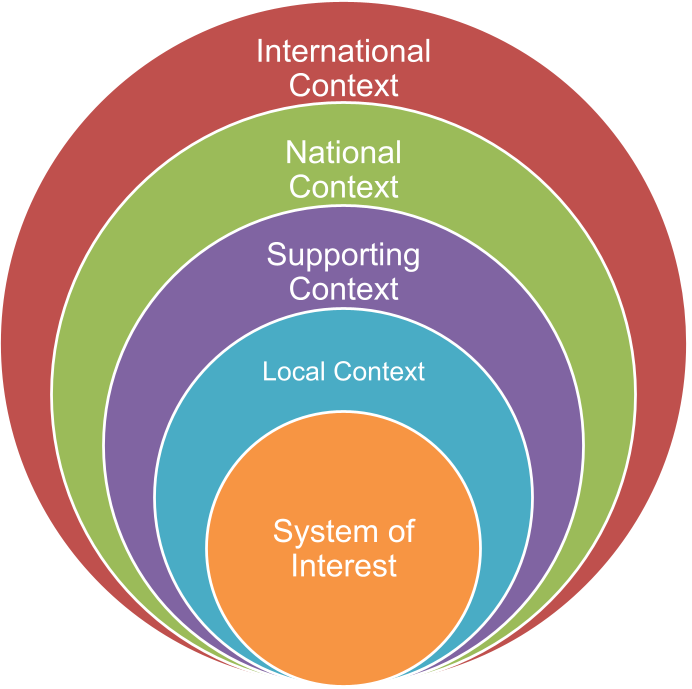
\includegraphics[width=0.4\textwidth]{Figures/chap3/scale.png}
\caption[Generic System Context Scales]{Generic System Context Scales}
\label{fig:scale}
\end{figure}

Dimensions meanwhile refers to the topical perspective taken within a Scale. There are innumerable potential such perspectives that one can take, but Figure \ref{fig:dimensions_generic} shows four basic ones that are commonly relevant in \ac{evdt} projects (and that roughly mean the \ac{evdt} questions discussed in Section \ref{sec:evdt-questions}). It also provides examples of the kinds of information that can be summarized with each Dimension.

\begin{figure}[!htb] 
\centering
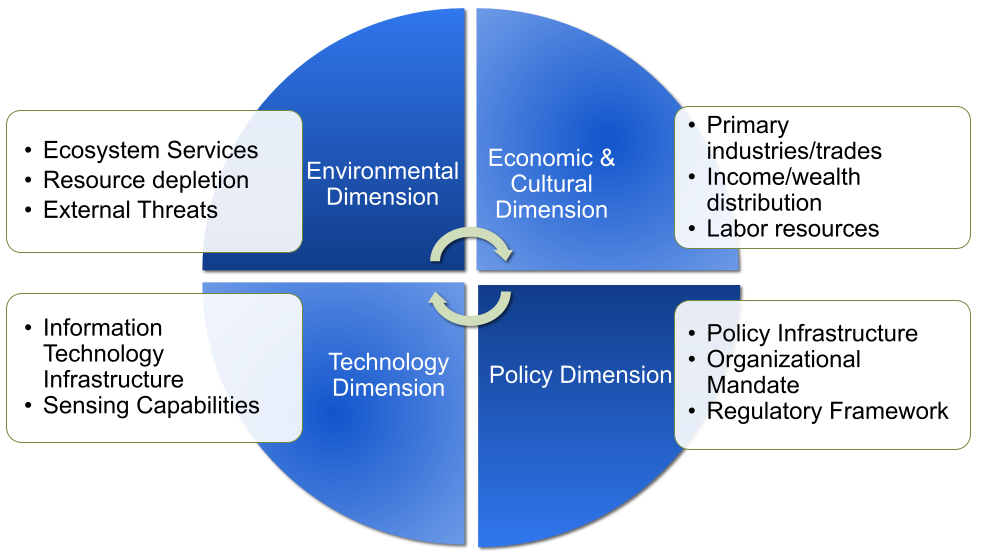
\includegraphics[width=0.7\textwidth]{Figures/chap3/dimensions_generic.png}
\caption[Generic System Context Dimensions]{Generic System Context Dimensions, including example items.}
\label{fig:dimensions_generic}
\end{figure}

Note that the most relevant dimensions may change as one progresses through the different Scales. Figure \ref{fig:dimensions_example} provides two examples. Each represents a different project and a different scale. The first is at the local scale for an \ac{evdt} project lead by Lombardo \cite{lombardoDevelopmentDecisionSupport2021, lombardoUtilizingSatelliteEarth2022}. It thus closely mirrors the generic case from above. The latter is at the national scale for a project looking at the creation of a new space agency \cite{woodBuildingTechnologicalCapability2012}. The relevant dimensions are thus quite different and even the dimensions that are similar (economic and technical) contain different types of information.

\begin{figure}[!htb] 
\centering
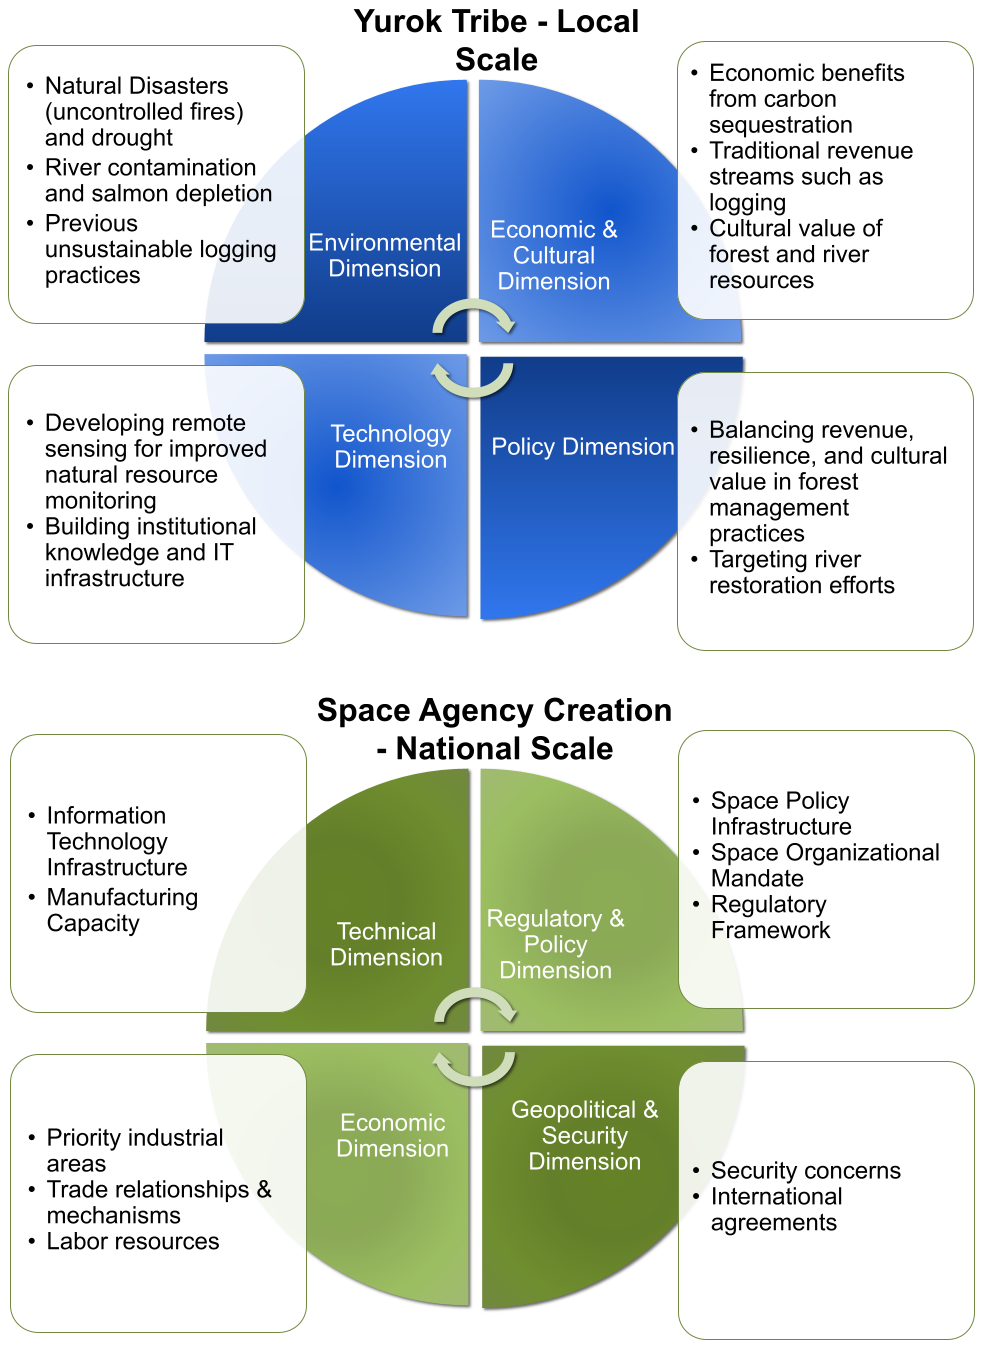
\includegraphics[width=0.7\textwidth]{Figures/chap3/dimensions_examples.png}
\caption[Example System Context Dimensions]{Example System Context Dimensions. \textbf{Top:} Four dimensions for the local scale Yurok tribe EVDT Project. Adapted from \cite{lombardoDevelopmentDecisionSupport2021}. \textbf{Bottom:} Four dimensions for the creation of a space agency at the national scale. Adapted from [**???]}
\label{fig:dimensions_example}
\end{figure} 


\subsubsection{\hlc[green]{Analyze System Stakeholders}} \label{sec:saf_stakeholders}

During the second \ac{saf} step, the various stakeholders, along with the relationships between them, are analyzed. This process may result in the identification of additional stakeholders or the decision to exclude stakeholders from consideration, though the latter should not be done lightly. The primary objectives of this step are (1) to understand how best to engage the stakeholders throughout the rest of the \ac{saf} and \ac{evdt} process; and (2) gain an understanding of how the Stakeholder Needs and Desired Outcomes overlap or conflict. The latter will be further examined in the next step.

A common initial approach for this step is to separate stakeholders into three categories: Primary, Secondary, and Tertiary, as shown in Table \ref{tab:primary-secondary-tertiary}. This approach, which draws on Crawley et al. \cite{crawleySystemArchitectureStrategy2015} and refined by Wood et al \cite{ovienmhadaInclusiveDesignEarth2021}, defines Primary Stakeholders as those who make direct decision on the design or operation of the system. Secondary Stakeholders are those who have direct influence on the Primary Stakeholders, typically via authority or funding. Tertiary Stakeholders are those that exert either little control or primarily indirect control on the system, but are impacted by the system. These are somewhat reductive categories and the listing of primary-secondary-tertiary should not be taken to understand a hierarchy of stakeholder worth or importance.

\begin{table}[!htb]
\caption[Primary-Secondary-Tertiary Classification of Stakeholders]{Primary-Secondary-Tertiary classification of stakeholders, including examples from \cite{ovienmhadaEarthObservationTechnology2020}}
\label{tab:primary-secondary-tertiary}
\begin{center}
\scriptsize
\begin{tabular}{ L{1.75cm} L{3.75cm}   L{3.75cm}  L{3.75cm} } \hline

& \textbf{Primary} & \textbf{Secondary} & \textbf{Tertiary}  \\ \hline

Description & Those who make direct decision on the design or operation of the system &  Those who have direct influence on the Primary Stakeholders, typically via authority or funding & Those that exert either little control or primarily indirect control on the system, but ae impacted by the system \\ \hline

Stakeholders & \tabitem \ac{gka} & 	\tabitem{National Institute of Water}
& \tabitem{People who participate in fishing or acadja practices} \\
& & \tabitem{\ac{gka} investors} & \tabitem{\ac{gka} harvesters} \\
& &	\tabitem{Benin government ministries} &	\tabitem{Lake Nokoue community and surrounding cities} \\ \hline
\end{tabular}
\end{center}
\end{table}

Other methods include both qualitative approaches such as flowchart creation or mapping, and more quantitative approaches such as Stakeholder Value Network Analysis \cite{fengDependencyStructureMatrix2010a} or agent-based modeling. The last of these is more relevant once Stakeholder Needs and Desired Outcomes have been identified. An example of stakeholder relational mapping can be seen in Figure \ref{fig:jaffe-stakeholder}. In its current form, it provided an excellent qualitative aid to understanding stakeholder relations, but it could also have been extended into a more quantitative Stakeholder Value Network Analysis if that had been considered useful.

\begin{figure}[!htb] 
\centering
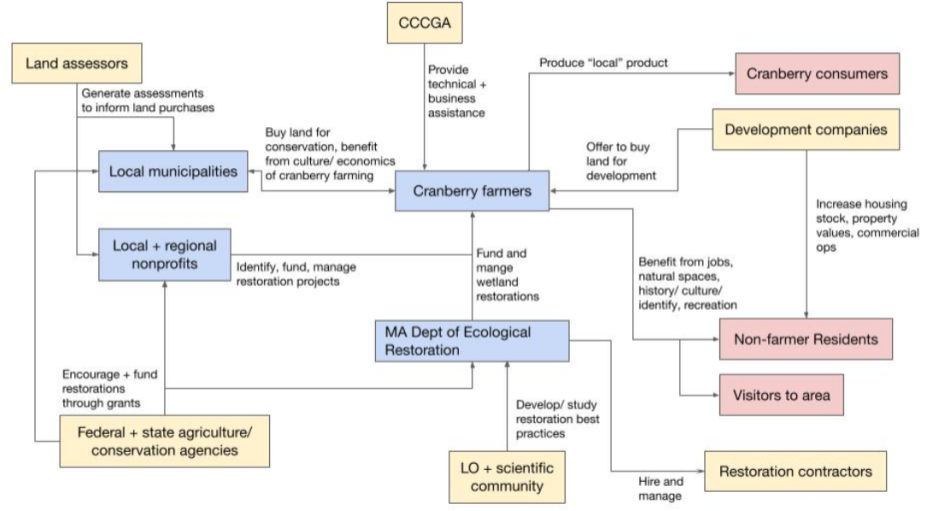
\includegraphics[width=0.9\textwidth]{Figures/chap3/jaffe-stakeholder.png}
\caption[Example stakeholder map of the Massachusetts Cranberry Industry]{Example stakeholder map of the Massachusetts Cranberry Industry. Figure from \cite{jaffeEnvironmentalEconomicSystems2022}}
\label{fig:jaffe-stakeholder}
\end{figure}

\subsubsection{\hlc[green]{Understand Desired Outcomes \& Objectives}}

Once both the System Context and the network of stakeholders are understood, we must next identify what the stakeholder Needs, Values, Desired Outcomes, and Objectives are.

System Needs refer to anything that a stakeholder is lacking. These are not necessarily tied to the system of interest. Desired Outcomes meanwhile are the end states that stakeholder would like to attain. Stakeholder Values are things that stakeholders hold as benefit in relation to needs and desired outcomes. It is important to note that Needs, Desired Outcomes, and Values do not exist in the abstract, but only when tied to a particular stakeholder, as shown in the example Table \ref{tab:need-outcome-objective}. This is a critical component of \ac{saf} and one of its major distinguishing characteristics compared to earlier applications of systems engineering to urban planning and development, as discussed at length in Sections \ref{sec:technocracy} and \ref{sec:se_critique}. They will vary from stakeholder to stakeholder, sometimes aligning in constructive ways and sometimes opposing one another. As a result, no singular, objective ``solution" will exist. Tradeoffs will need to be made and the system will serve the interests of some stakeholders more than others. The designer should be aware of this and honest about it.

One way to consider this is with the concept Architectural Alignment. This concept, which can be seen as the systems engineering version of a perspective of critique, asks, ``For what stakeholder or set of stakeholders does the system architecture constitute a satisfactory balance of preferences?" A poorly aligned system architecture may be the result of a compromise between some small number of stakeholders who have power over the system's design and operation. A well aligned system has some level of consensus and satisfaction among a wider set of stakeholders.

The goal of this step is to synthesize these Needs, Desired Outcomes, and Values, into (well aligned) System Objectives: the high level description of what the system will do. These can be quantitative or qualitative. Some sources use the term System Goals instead, in order to distinguish them from the optimization term ``objective function" \cite{nasaofficeofthechiefengineerNASASystemsEngineering2004}

\begin{table}[!htb]
\caption[Example Set of Needs, Outcomes, and Objectives]{Example set of Needs, Outcomes, and Objectives. Table from \cite{jaffeEnvironmentalEconomicSystems2022}}
\label{tab:need-outcome-objective}
\begin{center}
\scriptsize
\begin{tabular}{ L{1.75cm} | L{3.75cm} | L{3.75cm} | L{3.75cm} } \hline

\textbf{Stakeholder Group} & \textbf{Stakeholder Needs} & \textbf{Desired Outcomes} & System Objectives \\ \hline

Cranberry farmers & Make a sustainable living, recoup investment in land, provide for family & Improve profitability of farming or sell land for sufficient price, possibly keep land natural/open & Support/justify competitive sale pricing for land \\ \hline

MA Department of Ecological Restoration & Benefit people and the environment through restoration/protection of watersheds and wetlands; improve knowledge of restoration best practices & Widespread restoration/conservation of former cranberry farms; affordable and accessible restoration program & support/justify value of restoration projects; disseminate knowledge on restoration best practices; prototype novel funding models \\ \hline

Local municipalities & Provide clean drinking water, open/recreational space to citizens, address climate threats & Be able to provide high standard of safe, climate-resilient living to all residents & Support investment in projects/properties/programs that support clean water, open space, climate resilience \\ \hline

Local and regional nonprofits & Address risks of climate change and local environmental issues & Effective and affordable interventions to protect drinking water, become more climate resilient & Identify financing mechanisms, develop knowledge and best practices to support projects \\ \hline 

\end{tabular}
\end{center}
\end{table}

The methods described in the previous step for understanding relationships between stakeholders are also useful here to see how their needs, desires, and values overlap.

There are at least two schools of thought about how to approach balancing the needs of multiple stakeholders. One school argues for aggregating needs, values, and constraints into a singular objective function and set of constraints prior to considering any particular system functions or forms \cite{hazelriggFundamentalsDecisionMaking2012}. This can be done (a) unilaterally by the designer or a primary stakeholder; (b) through a reduction of all values to a common metric, often monetary \cite{viscusiEconomicsRegulationAntitrust2018}; or (c) through a negotiation process among the stakeholders. In general for the kinds of sustainable development applications that \ac{evdt} is envisioned to address, I suggest against this approach. Option (a) is essentially a return to the technocratic hubris criticized in Chapter 2. Option (b) is often difficult and morally problematic. It is difficult because many stakeholder values are difficult to reduce to monetary terms, particularly those values around the natural environment \cite{ackermanPricingPricelessCostBenefit2001}. While the field of ecosystem services (discussed further in Section \ref{sec:rio-vulnerability}) provides some help in this regard, such data is still sparse and unlikely to be comprehensive for a particular application. This option is also morally problematic because reducing values to monetary terms tends to prioritize the needs of wealthy stakeholders (who have more to lose) over economically poorer stakeholders. For example, if a designer is seeking to situate a seawall to reduce damages from cyclones, a purely monetary metric would suggest placing the seawall in front of large vacation homes instead of in front of smaller primary residences. If Option (b) is chosen, I strongly urge the designer to adjust values based on stakeholder wealth to more accurately capture actual impact on the stakeholder. This, of course, adds additional complexity. Option (c) in theory is fine, but many stakeholders will find it difficult to negotiate abstractly, without concrete alternatives available before them. This approach tends to reward those most familiar with fields that deal with the optimization of objective functions, such as systems engineering and economics. By choosing this option, the designer runs the risk of such stakeholders ``gaming the system." This is only worsened by the fact that such stakeholders are disproportionately likely to be in possession of other forms of power and authority.

The second approach is avoid making a unified objective function altogether or at the very least not to set the objective function in stone. Instead various concrete system objectives and form alternatives are proposed to stakeholders and compared in some form of negotiation or voting process. This option is preferred for most \ac{evdt} applications and is discussed further in the following two sections.  


\subsubsection{\hlc[green]{Select System Functions}}

During this step, the designer must refine System Objectives and use them to specify System Functions, the actions or processes that the system will perform to accomplish the Objectives.

Multiple techniques are available for coordinating input and involvement from various stakeholders, with varying levels of detail, time requirements, and balance of quantitative versus qualitative information. Many but not all have the person or persons facilitating the systems architecture process to conduct some form of negotiation process, supporting each of the stakeholders as needed. Examples include  multicriteria negotiations \cite{sparrevikUseMulticriteriaInvolvement2011},  pairwise comparison \cite{motieyanSustainableUrbanPlanning2017}, and various forms of the Delphi method \cite{morganUrbanPlanningUsing1979}. For an excellent survey of multicriteria decision-making analysis methods as applied to sustainable urban planning see Slattery, 2019 \cite{slatteryQuantitativeAssessmentSustainable2019}.

By moving stakeholder negotiations into this step (or even into the following step), the designer is able to provide more concrete examples to stakeholders, reducing the possibility of unforeseen consequences or misstated values. Where time and resources allow, it can be useful to iterate these negotiations at multiple phases: first when selecting System Objectives, again when defining System Functions, and a final time when designing the System Form.


\subsubsection{\hlc[green]{Assign Functions to Forms}} \label{sec:saf-assign}

The System Form is what a system is, rather than what it does. The System Form provides the instrument necessary for the System Functions. A particular bicycle is a Form that enables the Function of converting periodic human motion (pedaling) into linear motion (actually going somewhere).

The methods outlined in the previous section are largely still applicable here, as well as some additional approaches that depend on concrete system form alternatives, such as multi-stakeholder tradespace exploration \cite{fitzgeraldRecommendationsFramingMultistakeholder2016} and collaborative sketch planning \cite{vonkSociotechnicalPSSDevelopment2010}. When the system or system intervention is primarily a matter of a policy action, scenario planning workshops can be quite helpful for facilitating the expression of stakeholder preferences or even inducing stakeholders to generate new System Form proposals.

We generally recommend that Steps 1 through 5 be summarized in a concrete visual representation such as Figure \ref{fig:system-diagram}. These can be useful in describing the structure and dependencies within the system, as well as distilling the key aspects of the system in an easily understandable fashion. An alternative, list-based presentation can be seen in Ovienmhada et al. \cite{ovienmhadaInclusiveDesignEarth2021}.

\clearpage

\begin{figure}[!htb] 
\centering
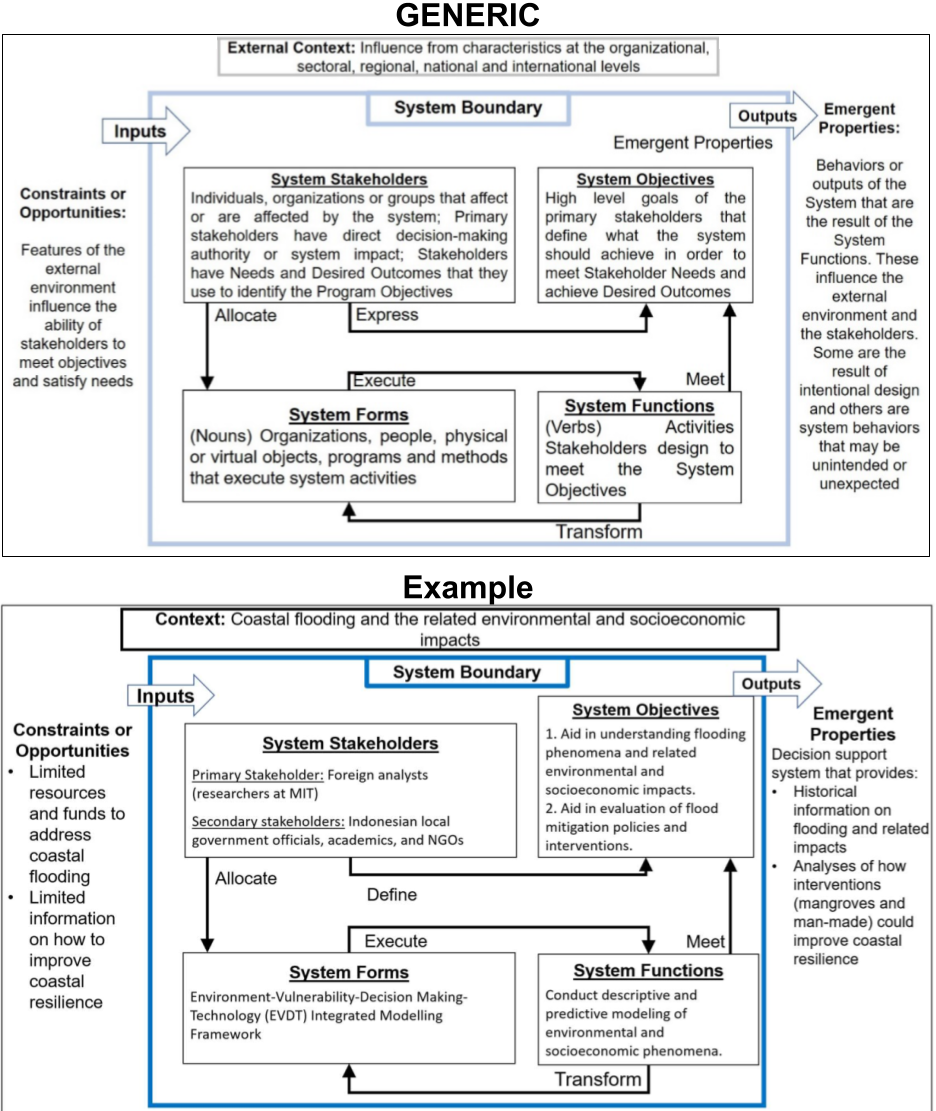
\includegraphics[width=0.9\textwidth]{Figures/chap3/system-diagram-combined.png}
\caption[Example system diagrams]{Example system diagrams. \textbf{Top:} Generic version. Credit to Danielle Wood. \textbf{Bottom:} Example from a coastal resilience \ac{evdt} project in Pekalongan, Indonesia. From \cite{lombardoEnvironmentVulnerabilityDecisionTechnologyFrameworkDecision2022}}
\label{fig:system-diagram}
\end{figure}

%%%%%%%%%%%%%%%%%%%%%%%%%%%%%%%%%%%%%5

%\begin{figure}[h] 
%\centering
%\includegraphics[width=0\begin{figure}[h] 
%\centering
%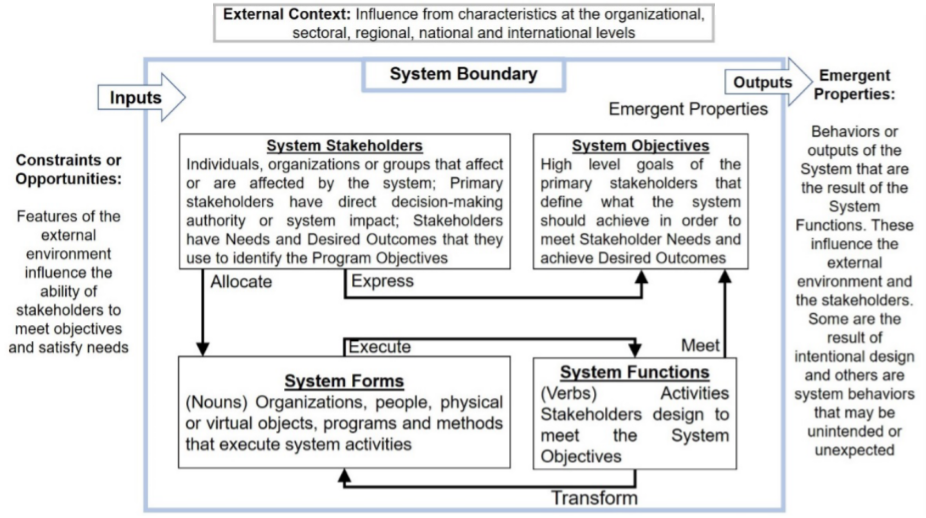
\includegraphics[width=0.9\textwidth]{Figures/chap3/system-diagram.png}
%\caption[Example system diagram]{Example system diagram. Credit: Danielle Wood}
%\label{fig:system-diagram}
%\end{figure}


\subsubsection{\hlc[green]{Monitor and Evaluate Systems}}

The sixth and final step of \ac{saf} directly leads back to the first. It is a statement that the work is never complete, the system never perfected. Perhaps the system will need to be monitored to ensure that it meets its objectives and further refined if it does not. Perhaps the objectives will change. Or perhaps an additional system needs to be developed to address some of the Stakeholder Needs and Desired Outcomes that went unaddressed in the original process. Either continuous or retrospective evaluations of the system should be conducted. The exact form of these will vary depending on the system at hand but can be as simple as surveying the various stakeholders. In our case, the output of the first iteration of the \ac{saf} leads directly into the third element of the \ac{evdt} Framework. Before getting to that, however, it is worth discussing why multiple iterations of the \ac{saf} are included in Figure \ref{fig:evdt_framework}.

\subsubsection{\hlc[cyan]{A Note on Perspective}}

As implied in the section ``Understand System Context" above, there is a certain level of arbitrariness in defining the System Boundary. This choice affects what stakeholders are included, which stakeholder(s) are made central (if any), and has significant impact on the system objectives, functions, and forms.

When time and resources allow, it can be useful to consider the system from multiple different perspectives before settling on any particular one. As shown in Figure \ref{fig:evdt_framework}, for an application of the \ac{evdt} Framework, I suggest going through the \ac{saf} at twice. The first, Iteration 1, is a purely descriptive process, detailing how the system of interest currently operates.  The second, Iteration 2, which will leverage the above suggested methods more fully, is then used for developing the design of the new system or intervention, be it a product, service, or policy. In projects involving the creation of a \ac{dss} (which \ac{evdt} Framework projects are), the differences between Iteration 1 and Iteration 2 can also help to distinguish the objectives, functions, and form of the \ac{dss} versus the objectives, forms, and functions of the system that the \ac{dss} is supporting decisions about.

It can also be worthwhile to conduct a separate iteration of the \ac{saf} between Iterations 1 and 2 (call this Iteration 1.5). In this iteration, situate the designer or the designers organization as the primary stakeholder. In the case of this thesis, that would be Space Enabled and/or myself. This allows the designer to clearly identify their own personal interests and objectives in the project, rather than to pretend they are a purely altruistic agent (which is rarely the case).
By comparing the results of Iteration 1 and Iteration 2 with Iteration 1.5, the designer can assess whether or not this project is a good fit for themself. If their own Needs and Desired Outcomes differ too greatly from those of the other stakeholders, it may be best to not pursue the project. See Section \ref{sec:se_critique} for further discussion of what can occur when a system designer's personal research goals take priority over those of the other stakeholders.





\subsection{\hlc[cyan]{B: EVDT Questions \& Models}} \label{sec:evdt-questions}

The \ac{evdt} Framework conceptualizes the application system from two different perspectives. The first is the system boundaries and stakeholders perspective from \ac{saf} shown in Figure \ref{fig:saf} and discussed in Section \ref{sec:saf}. The second perspective focuses on combining the established fields of sociotechnical systems \cite{rouseUnderstandingChangeComplex2012,siddiqiSociotechnicalSystemsSustainability2017,sussmanTeachingComplexSociotechnical2010} and socio-environmental systems \cite{elsawahEightGrandChallenges2020} into \ac{sets}. To accomplish this, at least four components are considered: the Environment (data including Landsat, Sentinel, VIIRs, in-situ environmental data and knowledge, etc.); Human Vulnerability and Societal Impact (data including census and survey-based demographic data, eocsystem services valuations, NASA's Socioeconomic Data and Applications Center, local knowledge of impacts, etc.); Human Behavior and Decision-Making (data including policy histories, mobility data, urban nightlight data, community input, etc.); and Technology Design for earth observation systems including satellites, airborne platforms and in-situ sensors (data including design parameter vectors for such systems). The data from each of these domains is used by established models in each domain, which are adapted to work in concert to address the objectives identified with the \ac{saf} and develop the \ac{dss} discussed later in Section \ref{sec:dss}. The four components, shown in Figure \ref{fig:model}, seek to encapsulate the major interacting aspects of sustainable development and consider them from a \ac{sets} perspective. 

\begin{figure}[!htb]
    \centering
    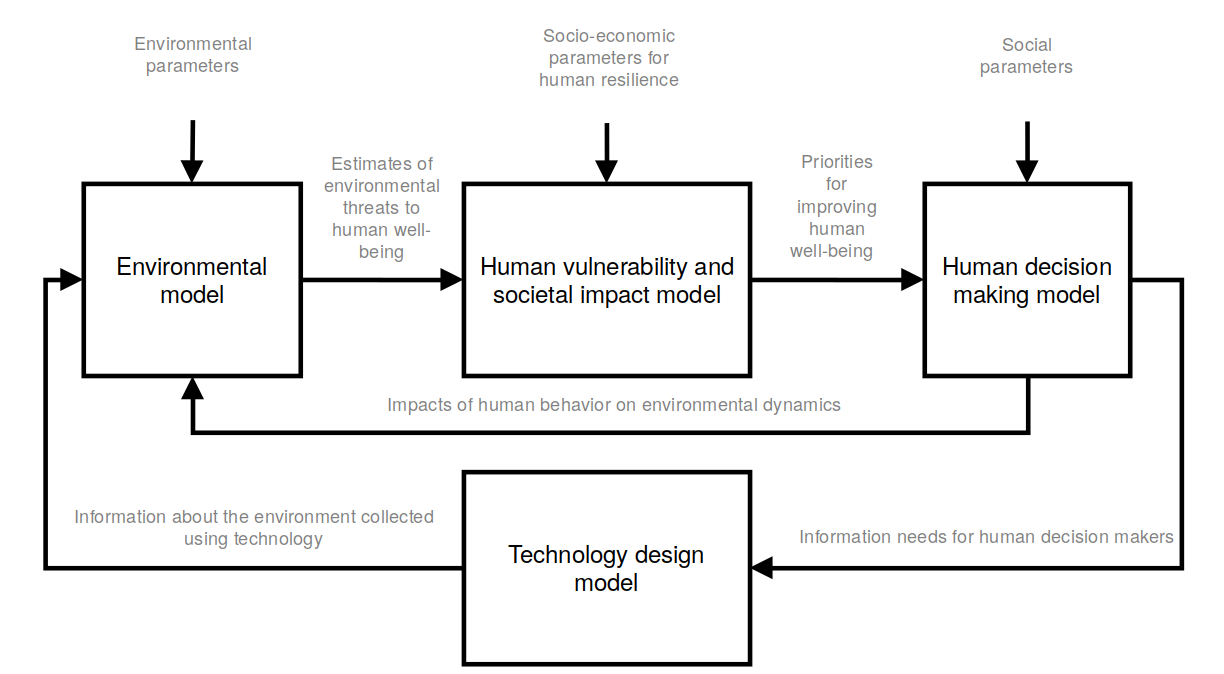
\includegraphics[scale=0.3]{Figures/chap3/modelflow.png}
    \caption[Generic version of EVDT Model] {Generic version of the Environment - Vulnerability - Decision - Technology Model}
    \label{fig:model}
\end{figure}

There are specific advantages to this perspective. As discussed in Section \ref{sec:sustainable_development}, jointly considering these four aspects is key to a proper understanding of sustainable development. Sachs used a similar framing when he wrote: ``Sustainable Development involves not just one but four complex interacting systems. It deals with a global economy...; it focuses on social interactions...; it analyzes the changes in complex Earth systems...; and it studies the problems of governance" \cite{sachsAgeSustainableDevelopment2015}. This is slightly different from \ac{evdt} to be clear. Sachs focuses specifically on a economics where \ac{evdt} more broadly considers vulnerability and societal impact. Sachs also, not unreasonable, breaks decision-making into two categories: social interactions and governance. Finally Sachs omits the role of technology in this list, though elsewhere he acknowledges that ``technology road-mapping" is critical for the pursuit of sustainable development.

Such an approach, which seeks to simultaneously consider both humans and the environment, stands in contrast to some historical categorizations of planning models. Clifton et al., for instance, breaks down the various ways of modeling the urban form into five categories (though they do not assert that these are comprehensive), as seen in Table \ref{table:urban_form} \cite{cliftonQuantitativeAnalysisUrban2008}. Notably, each model ``perspective" is associated with a ``principal concern" and ``disciplinary orientation" that seems to exclude the others. An \ac{evdt} approach argues that each of these modeling perspectives must be considered simultaneously as problems as ``environmental protection, economic efficiency, accessibility, social welfare, and aesthetics." This is not to say that every \ac{evdt} \ac{dss} must simultaneously model landscape ecology and transportation planning, but it should acknowledge the various (competing or cooperating) concerns. While \ac{evdt} does not focus specifically on urban form, it is interested in these types of models, with the case studies presented in this work focusing on landscape ecology and community design in particular. One downside of examinations of urban form is that they tend to focus on areas and residences, while various forms of social exclusion are better measured by focusing on individuals instead \cite{scottRoleUrbanForm2008}.

\begin{table}[!htb]
\begin{center}
\scriptsize
\caption[Five categories of urban form models]{Five categories of urban form models. Adapted from \cite{cliftonQuantitativeAnalysisUrban2008}}
\label{table:urban_form}
\begin{tabular}{ L{2cm} L{2cm}  L{2cm} L{2cm} L{2cm} L{2cm}} \hline
Perspective & Principal concern & Disciplinary Orientation & Scale & Nature of Data & Common Metrics  \\ \hline

Landscape ecology & Environmental protection & Natural scientists & Regional & Land cover & Land cover change; Contagion \\ 

Economic structure & Economic efficiency & Economists & Metropolitan & Employment and population & Density gradient; Land value  \\

Transportation planning & Accessibility & Transportation planners & Submetropolitan & Employment, population and transportation network & Expected travel time; capacity  \\

Community design & Social welfare & Land-use planners & Neighborhood & Local \ac{gis} data & Proximity to needs; Zoning; Accessibility \\

Urban design & Aesthetics and walkability & Urban designers & Block face & Images, surveys, and audits & Lot size; Accessibility \\ \hline
\end{tabular}
\end{center}
\end{table}

The set of four models with the particular linkages shown in Figure \ref{fig:model} are not the only form that \ac{evdt} can take, merely the most general arrangement. Some applications may involve replacing a model with a human-in-the-loop (e.g. having the user themself substitute for the decision-making model) or omitting a model altogether. For other applications, it may make sense to conceptually break a model into two or more components. In the Vida project, it was considered worthwhile to separate the social impact model into two components, one focusing on public health (the obvious priority when dealing with \ac{covid}) and one focusing on non-health metrics (such as income, employment, etc.). Such a separation can be useful if either significantly different modeling methodologies are going to be used or if the linkages with the other \ac{evdt} components are different from one another. 

One way to determine the optimal arrangment of \ac{evdt} components is to consider what questions the user or researcher is seeking to answer with this application of \ac{evdt}. For instance, the default \ac{evdt} arrangement shown in Figure \ref{fig:model} was motivated primarily by the following four questions:

\begin{enumerate} \setlength{\itemsep}{0pt} \setlength{\parskip}{0pt}
    \item What is happening in the natural environment?
    \item How will humans be impacted by what is happening in the natural environment?
    \item What decisions are humans making in response to environmental factors and why?
    \item What technology system can be designed to provide high quality information that supports human decision making?
\end{enumerate}

Alternate questions may result in a different configuration or set of components (further discussion of this in Section \ref{sec:intended}). The point of \ac{evdt} is not to insist upon a particular set of linkages and feedbacks, but rather to encourage a consideration of such linkages between domains in general, and to consider them through a systems engineering perspective. Of course answering the structuring questions, and even phrasing them in the first place, requires the use of collaborations.

\subsection{\hlc[cyan]{C: Interactive Decision Support System}} \label{sec:dss}

Ultimately, the goal of the two \ac{saf} iterations and E-V-D-T framing is to develop an interactive \acf{dss} to inform community decision-making on the topic of sustainable development.

A key aspect of the term \ac{dss} is the word "support." Crawley et al. state that the goal of a \ac{dss} is to "\emph{enhance} the efficiency of decision makers by providing tools to quantitatively and qualitatively explore a space of alternatives for single or multiple decisions" [emphasis added] \cite{crawleySystemArchitectureStrategy2015}. This means that the \ac{evdt}-developed \ac{dss} should not present decisions as a \textit{fait accompli} but instead support stakeholders in developing their own solutions. Ideally this means that individual stakeholders can directly handle and explore any simulations or models used, along with their underlying assumptions and structure. If this is not feasible, an indirect form of interaction can be used, such as when a stakeholder provides verbal instruction to someone who then implements that instruction in the \ac{dss}. The latter option can be quite useful when there are barriers of language, familiarity, or technical knowledge, and is commonly used in purposeful gaming \cite{rossGamebasedLearningSystems2014}, wargaming \cite{hansonImprovingOperationalWargaming2016,selvaRevitalizingWargamingNecessary15,shlapakReinforcingDeterrenceNATO2016}, and role playing gaming \cite{groganStrategicEngineeringGaming2012,groganFederatedSimulationGaming2012}. Additionally, in contrast to Crawley's definition which centers on the ``efficiency of decision-makers," (see the concerns raised in Section \ref{sec:elitism}) I argue that an ideal \ac{dss} should cause a decision-maker to consider multiple perspectives (such as the four models of \ac{evdt} and those of other stakeholders) and thereby make \textit{better} decisions as well.

The form and functions of the \ac{dss} may vary significantly and should be based on the results of the \ac{saf} iterations. Regarding form, both of the case studies discussed in this work (Chapters \ref{ch:mangroves} and \ref{ch:vida}) present desktop-based computer applications. Jaffe used a web-based application, showin in Figure \ref{fig:jaffe_application} (the full application is, at time of writing, available at \url{https://cranberry-land-use-explorer.herokuapp.com/}) \cite{jaffeEnvironmentalEconomicSystems2022}. Another potential form includes paper maps and other forms of data used as part of an interactive session. Note that paper maps are not, in and of themselves interactive, and they run the risk of merely presenting a solution to the stakeholders rather than engaging them to make a decision. In general, \ac{evdt} takes a somewhat Harleian approach to visualization, in which ``\textit{presentation} is de-emphasized in favor of \textit{exploration} of data" \cite{cramptonMapsSocialConstructions2001}.

\begin{figure}[!htb]
	\centering
	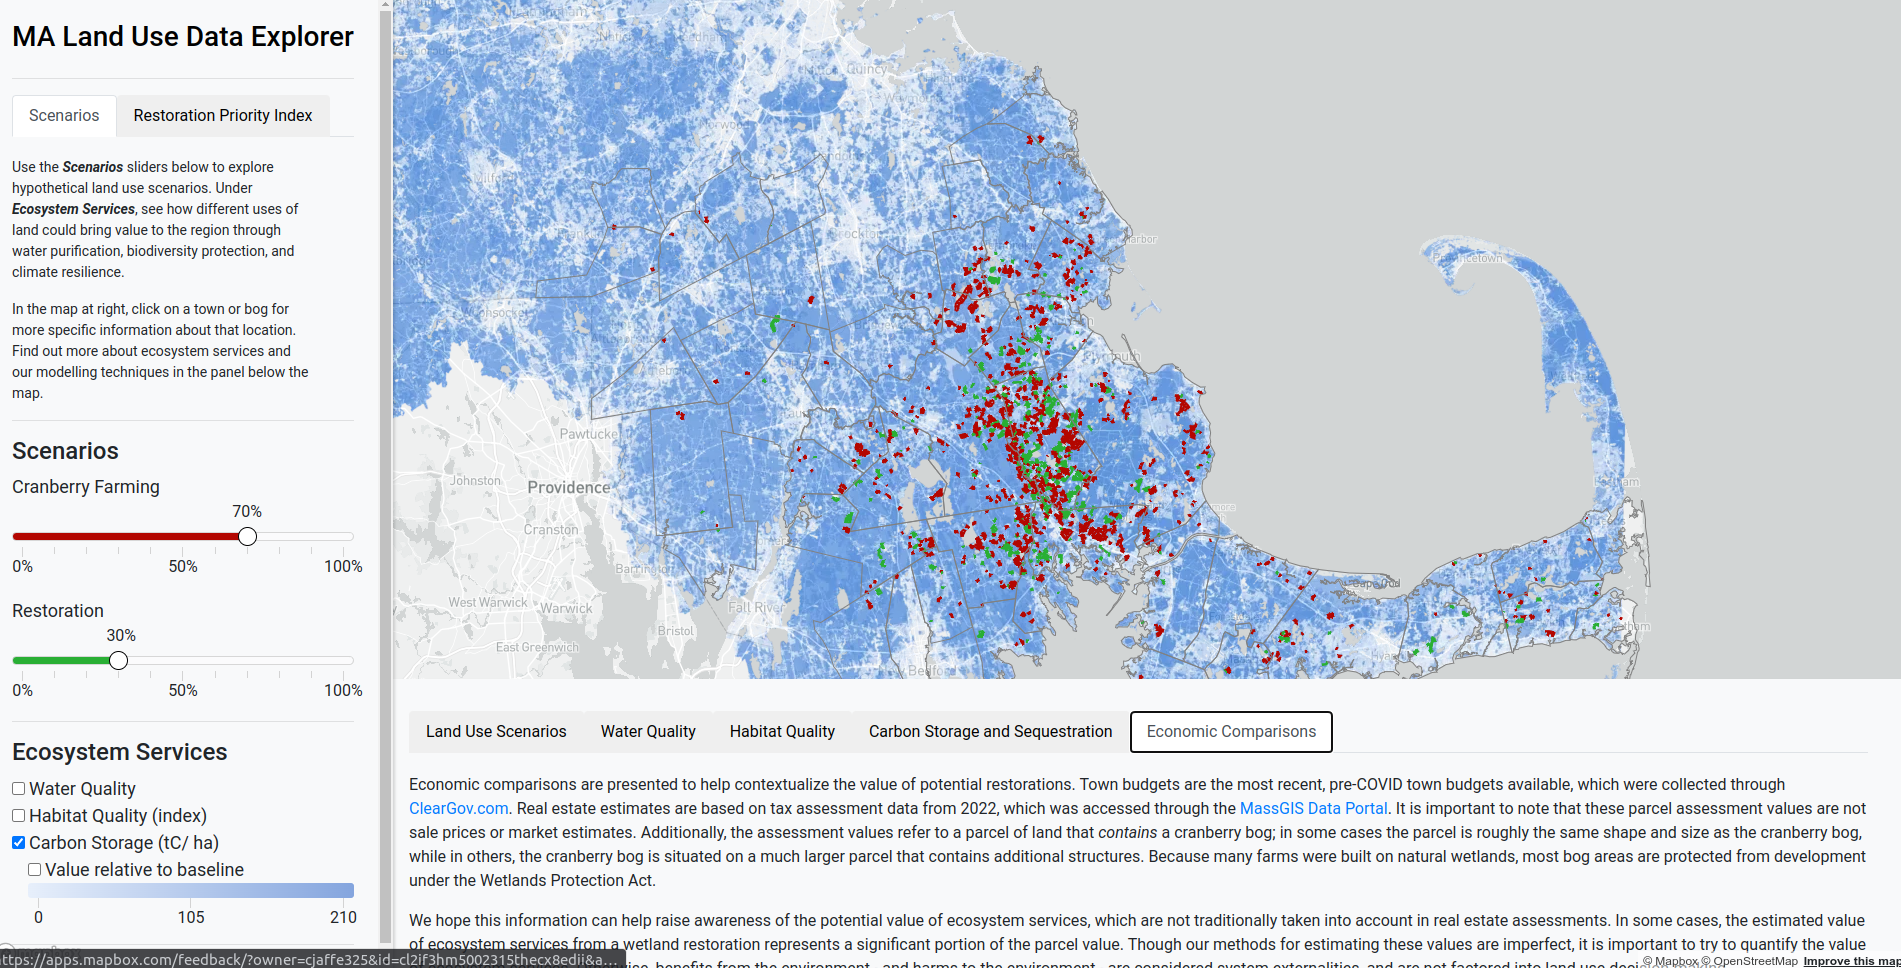
\includegraphics[scale=0.2]{Figures/chap3/jaffe_application.png}
	\caption[Screenshot of Jaffe's Decision Support System] {Screenshot of Jaffe's Decision Support System. See \cite{jaffeEnvironmentalEconomicSystems2022} for more information.}
	\label{fig:jaffe_application}
\end{figure}

It should be noted recognized that offline \acp{dss} (be they come in the form of desktop software or pen-and-paper) come with numerous downsides. \textit{theirwork}, an early collaborative, open source \ac{gis} platform, specifically "decided at an early stage to make the software Web-based to allow for a process of rapid development and iteration and allow a maximum number of potential participants." \cite{williamsonTheirworkDevelopmentSustainable2011} This is not universally true, however. \textit{theirwork} was a UK-based project (an area with high internet connectivity penetration) and started in the mid 2000's, a period with significantly less diversity of internet browsing methods compared to nowadays, which simplified the task of ensuring accessibility. Nonetheless, it is impossible to deny the collaboration and software sustainability benefits of an online platform, particularly in an age when many of the early concerns with the internet (low speeds, lack of knowledge about how to use it, etc.) \cite{shifterInteractiveMultimediaPlanning1995} have been largely alleviated.

If a web app or some other form is chosen such that a user might engage with the \ac{dss} individually, the \ac{dss} should include all necessary information to provide both instruction in its use and context for the information presented. Jaffe's \ac{dss} does just this, providing instruction in the top left and contextual information across the bottom. \acp{dss} intended for use in group workshops or with guidance can contain less of both instruction and context.

Regarding function, the case study presented in Chapter \ref{ch:vida} does some in-app computation and simulation based on user inputs. This is preferred when the potential set of user inputs is quite vast and live computation able to be performed quickly. For Jaffe's \ac{dss}, meanwhile, she pre-computed all potential outcomes and the \ac{dss} simply presents those outcomes on demand. This is preferred when the potential set of user inputs is restricted (in Jaffe's case, there are ten possible user inputs) and/or computational speed of the models would be quite slow (as it was in Jaffe's case). 

Generally an \ac{evdt} \ac{dss} should include some presentation of \ac{gis} data, be it raster data derived from \ac{eo} imagery or vector demographics data. Choropleths are one of the more common types of non-imagery geospatial data used in \ac{evdt} projects. These are maps that express "quantity in area" (i.e. some statistic tied to a particular geographic area with color, texture, or shading). It should be noted that choropleths have a few well-known limitations, including the ecological fallacy and the modifiable areal unit problem \cite{cramptonRethinkingMapsIdentity2011, sawickiNeighborhoodIndicatorsReview1996}. It is for these reasons that \ac{evdt} does not rely entirely on choropleths and why we strive to store data with the finest geospatial resolution available. This is also why, when possible, a zoom function should be provided so that users can focus on particular subsets of the map that are of interest (such as their home or workplace). While three dimensional data exists for both the urban environment \cite{battyVisualizingCityCommunication2000} and from remote sensing \cite{sunAerial3DBuilding2013}, \ac{evdt} projects to date have focused primarily on two dimensional symbolic visualizations.

Historically, \ac{gis} implementations have often struggled to handle temporal data \cite{harrisLocationalModelsGeographic1993}. For this reason the \ac{dss} should not be limited to presenting information in the form of maps. Timelines, graphs, and timelapses may all be relied upon to present changes over time.

All of this points to a general rule of thumb regarding \ac{evdt} \acp{dss}: Do not neglect visual aesthetics and usability. Technologists often focus on the underlying models and the ``interesting" technical problems. The point of the \ac{evdt} Framework is not to make a \ac{dss}. The \ac{dss} is a means of helping communities to make decisions. In most \ac{evdt} projects, at least some stakeholders will not be \ac{gis} experts or professionals. Care must be taken so that the visualization is easily understandable by a lay audience. Batty et al. refers to this as the distinction between \textit{backward visualization}, which focuses on developing tools for experts and professionals, and \textit{forward visualization}, which supports decision-making by a less (\ac{gis}-)informed constituency, including the public \cite{battyVisualizingCityCommunication2000}.

For example, initial \ac{evdt} projects featured quite large graphics. Tufte argues that graphics in general should be significantly shrunk and that "many data graphics can be reduced in area to half their current published size with virtually no loss in legibility and information." \cite{tufteVisualDisplayQuantitative2001} In accordance with this Shrink Principle, these graphics were greatly reduced in later versions. 

In general, care should be taken in making fundamental architectural decisions in the development of the \ac{dss}. As with most \ac{gis} software \cite{heikkilaGISDeadLong1998}, early \ac{evdt} projects were structured as entirely object-oriented, and later versions remained primarily object-oriented. This has many advantages but also comes at certain costs, the most important of which include (a) difficulty in recording continuous spatial variables and (b) a requirement to pre-identify the different classes (objects) to sort phenomena and relationships into \cite{goodchildModelingEarth2011}. Similarly care, must be taken such that the form of the \ac{dss} supports the circumstances in which it will be used. Jankowski proposed four different kinds of meeting arrangements, shown in Table \ref{table:meeting_arrangements}, each with their advantages and disadvantages. Not all \acp{dss} forms are equally suited for each of these arrangements.

\begin{table}[!htb]
\caption[Different types of meeting arrangements]{Different types of meeting arrangements. Adapted from \cite{jankowskiGISGroupDecision2001}}
\label{table:meeting_arrangements}
\begin{center}
\footnotesize
\begin{tabular}{ L{2cm} L{6cm}  L{6cm}}  \hline
 & \textit{Same time} &\textit{Different time}  \\ \cline{2-3}
\textbf{\textit{Same place}} & \textbf{Conventional Meeting} \qquad \textit{Advantage:} 
\vspace{-3mm}
\begin{itemize}[itemsep=0pt,parsep=0pt]
    \setlength{\itemsep}{0pt}%
    \setlength{\parskip}{0pt}%
	\item{face-to-face expressions}
	\item{immediate response}
\end{itemize} &
\textbf{Storyboard meeting} \qquad \textit{Advantage:}
\vspace{-3mm} 
\begin{itemize}[itemsep=0pt,parsep=0pt]
    \setlength{\itemsep}{0pt}%
    \setlength{\parskip}{0pt}%
	\item{scheduling is easy}
	\item{respond anytime}
	\item{leave-behind note}
\end{itemize} 
\\
& \textit{Disadvantage:} 
\vspace{-3mm}
\begin{itemize}[itemsep=0pt,parsep=0pt]
    \setlength{\itemsep}{0pt}%
    \setlength{\parskip}{0pt}%
	\item{scheduling is difficult}
\end{itemize} &
\textit{Disadvantage:} 
\vspace{-3mm}
\begin{itemize}[itemsep=0pt,parsep=0pt]
    \setlength{\itemsep}{0pt}%
    \setlength{\parskip}{0pt}%
	\item{meeting takes longer}
	\item{difficult to maintain in the long run}
\end{itemize} 
\\ \hline

\textbf{\textit{Different place}} & \textbf{Conference call meeting} \qquad \textit{Advantage:} 
\vspace{-3mm}
\begin{itemize}[itemsep=0pt,parsep=0pt]
    \setlength{\itemsep}{0pt}%
    \setlength{\parskip}{0pt}%
	\item{no need to travel}
	\item{immediate response}
\end{itemize} &
\textbf{Distributed meeting} \qquad \textit{Advantage:} 
\vspace{-3mm}
\begin{itemize}[itemsep=0pt,parsep=0pt]
    \setlength{\itemsep}{0pt}%
    \setlength{\parskip}{0pt}%
	\item{scheduling is convenient}
	\item{no need to travel}
	\item{submit response anytime}
\end{itemize} 
\\
& \textit{Disadvantage:} 
\vspace{-3mm}
\begin{itemize}[itemsep=0pt,parsep=0pt]
    \setlength{\itemsep}{0pt}%
    \setlength{\parskip}{0pt}%
	\item{limited personal perspective from participants}
	\item{meeting protocols are difficult to interpret}
	\item{difficult to maintain meeting dynamics}
\end{itemize} &
\textit{Disadvantage:} 
\vspace{-3mm}
\begin{itemize}[itemsep=0pt,parsep=0pt]
    \setlength{\itemsep}{0pt}%
    \setlength{\parskip}{0pt}%
	\item{meeting takes longer}
	\item{meeting dynamics are different from normal meeting ("netiquette" instead of face-to-face etiquette)}
\end{itemize} 
\\ \hline
\end{tabular}
\end{center}
\end{table}


\subsection{\hlc[cyan]{D: Re-use \& Community Development}} \label{sec:reuse}

One of the limitations with some of the previous and current work discussed in Section \ref{sec:gap}, was a focus on solving a particular problem with little attention paid to how to scale or generalize the approach to other problems. This is one of the key benefits of a framework such as \ac{evdt}. This section explains how \ac{evdt} approaches such scaling beyond an individual problem.

One of the key motivations of participatory, stakeholder-involved processes is capacity building. In the case of the \ac{evdt} Framework, this includes both capacity building in a specific application community and in the broader practitioner community of those using \ac{eo}, \ac{gis}, and systems engineering for sustainable development. Both ends are served by designing the \ac{dss} with re-use and modularity in mind. The ability to track mangrove health in Brazil \cite{reidInteractiveModelAssessing2020} proved to be useful in a later application in Indonesia \cite{lombardoEnvironmentVulnerabilityDecisionTechnologyFrameworkDecision2022}. 

The intent is not for this team to develop complete, black-box products, but rather to facilitate the the tool development process for others. Part of this includes the co-design requirement, but another part is making the code itself readily available online and designing the implementation of the framework to be as reusable as possible. In this way, users in a new context may be able to reuse previous \ac{eo} data processing techniques, while focusing on the vulnerability or decision-making components. This is also important to provide clarity on ultimate ownership and responsibility for the product.

The second form of capacity building is pursued by developing a community of practice around \ac{evdt} and related endeavors. This includes enabling ``peer-to-peer" interactions where representatives of a community involved in an \ac{evdt} project may directly correspond with those from other projects. To this end, the Space Enabled team has been hosting approximately monthly meetings with open invites to all those currently involved in \ac{evdt} projects and those interested in becoming involved. These meetings started as part of the Vida project (discussed more in Chapter \ref{ch:vida}) before transitioning into a broader focus on \ac{evdt} projects in general. In the future we would like to have other means of interaction, such as in-person meetings, an online system for sharing information, and more one-to-one meetings that may not involve Space Enabled at all.

\subsection{\hlc[cyan]{E: Collaborative Development}} \label{sec:evdt-collab}

While the \ac{saf} specifies that the relationships and perspectives of multiple stakeholders are considered, it does not explicitly call for their participation in the development process. The \ac{evdt} Framwork, however, does. It is worth explaining exactly what this entails.

Involving stakeholders in the development process, in addition to the requirements definition process, is key for ensuring adoption and capacity building. This has been recognized by the \ac{pgis} movement, which increasingly emphasizes the importance of open source software \cite{williamsonTheirworkDevelopmentSustainable2011, dodgeMappingModesMethods2011}. It is also core to the Data Action framework which, responding to the idea that "data is never raw, it's collected," emphasizes the use of participatory and collaborative methods for collecting and using data \cite{williamsDataActionUsing2020}. The history of this trend along with the various benefits, both practical and ethical, of the participative approach, were discussed at length in Section \ref{sec:collaborative}, \ref{sec:elitism}, \ref{sec:scenario_critique}, and \ref{sec:chap2-conc}.

Collaborative development is increasingly feasible as barriers have dropped over the past couple of decades. Knowledge and familiarity with computers and programs has expanded, access to sufficient hardware is increasingly common (particularly with the rise of cloud computing platforms), and both synchronous and asynchronous online collaboration tools have proliferated. Obviously such barriers have not been universally eliminated. Furthermore, even in the absence of barriers, not everyone desires to be a computer programmer, earth scientist, \ac{eo} specialist, or social scientist, even part-time (and the world is better for it!). Collaborative development must therefore take different forms in each project, being as welcome as possible to all while accommodating stakeholder preferences and constraints.

The \ac{evdt} Framework invites participation in different forms throughout the process.

\begin{enumerate} \setlength{\itemsep}{0pt} \setlength{\parskip}{0pt}
    \item{\textbf{Pre-Project:} Ideation through the initial, tentative definitions of the System Boundary. An \ac{evdt} project should not be conceived without some active interest from one or more local stakeholder \footnote{See \textit{Local Context Expert} in Section \ref{sec:intended}.}.  The more local the better (i.e. a resident or member of a municipal government is to generally to be preferred over a national government minister). This initial contact should not be assumed to be the sole representative of the community but they are integral to starting to grapple with the system of interest.}
	\item{\textbf{\ac{saf} Iterations:} This is discussed throughout Section \ref{sec:saf}. It is the stage at which a wider set of stakeholders are identified, contacted, solicited for perspectives, and invited for further participation.}
	\item{\textbf{Development of the \ac{dss}:} This refers to the implementing of the forms and functions identified during the \ac{saf} iterations, the actual coding or creation of the \ac{dss}, including its various constituent models. This typically requires some minimum level of technical knowledge, but do not dismiss local expertise even when they lack some university degree. They are typically the only ones with the requisite knowledge of what assumptions to make in the models, how to go about validating models as necessary, what regional datasets might be available, and how to translate terminology\footnote{Even if you know the primary language spoken by the community, do not assume that all terms are used identically. For example, during the case study in Chapter \ref{ch:mangroves}, I initially translated ``mangrove health" into Portuguese as ``saúde do mangue," only to find out (by asking) that locals tended to use the phrase ``qualidade de mangue" instead. This lead to a productive conversation about the distinctions between these phrases and which had the preferred connotation for use in the \ac{dss}.}. Interest in participating in the actual programming of the \ac{dss} (in the cases where the \ac{dss} is software) should be encouraged. For those with previous coding experience, numerous platforms, both asynchronous and synchronous exist to allow for collaboration, be it in-person or remote. For those who lack such experience, sufficient coding educational resources are available to help instruct a novice as necessary. Do not begrudge the extra time and effort as the goals is to not make a \ac{dss} for its own sake, but to assist the community in making its own decisions.}
	\item{\textbf{Deploying and Evaluating the \ac{dss}:} Ideally ``possession" of the resulting \ac{dss} should not reside with a particular stakeholder but instead be available to any with interest. This can include passive means such as deploying a web app (though make sure to advertise its existence) or more active means such as organizing scenario planning workshops or directly soliciting feedback.}
	\item{\textbf{Ongoing Collaboration with the \ac{evdt} Community:} Participants in one \ac{evdt} project should be encouraged to participate in others. This is discussed further in \ref{sec:reuse}.}
\end{enumerate}

The \ac{evdt} Framework also certainly builds upon Jankowski's and Nyerges' macro-micro strategy for participatory decision-making \cite{jankowskiGISGroupDecision2001}. This strategy, shown in Table \ref{tab:macro-micro}, envisions decion-making as taking place across three macro-phases (Intelligence, Design, and Choice), each of which are made up of an iteration of the same four micro-activities (Gather, Organize, Select, and Review). The first iteration of the \ac{saf} is essentially a specific approach for accomplishing Phase 1A through 2A. The second iteration of \ac{saf} results in the creation of a \ac{dss} that in turn supports the community in accomplishing Phase 2B through 3D. 

\begin{table}[!htb]
\footnotesize
\caption[Generic macro-micro, participatory decision strategy]{Generic macro-micro, participatory decision strategy. Adapted from \cite{jankowskiGISGroupDecision2001}}
\label{tab:macro-micro}
\begin{center}
\begin{tabular}{ L{2.5cm} L{3.5cm}  L{3.5cm} L{3.5cm}} \hline
& \multicolumn{3}{c}{\textit{Macro-phases in a decision strategy}}  \\ \cline{2-4}

\textit{Micro-activities in a decision strategy} & \textbf{\textit{1. Intelligence}} about values, objectives, and criteria & \textbf{\textit{2. Design}} of a set of feasible options &  \textbf{\textit{3. Choice}} about recommendations \\ \hline

\textbf{A. Gather...} & issues to develop and refine \textbf{value trees} as a basis for objectives & \textbf{primary criteria} as a basis for option generation & \textbf{values, criteria, and option list scenarios} for an evaluation \\ \hline

\textbf{B. Organize...} & \textbf{objectives} as a basis for criteria and constraints & and apply approaches(es) for \textbf{option generation} & approaches to \textbf{priority and sensitivity analyses} \\ \hline

\textbf{C. Select...} & \textbf{criteria} to be used in analysis as a basis for generating options & the \textbf{feasible option list} & \textbf{recommendation} as a prioritized list of options \\ \hline

\textbf{D. Review...} & criteria, \textbf{resources, constraints,} and \textbf{standards} & \textbf{option set(s)} in line with resources, constraints, and standards & \textbf{recommendation(s)} in line with original \textbf{value(s), goal(s),} and \textbf{objectives} \\ \hline

\end{tabular}
\end{center}
\end{table}

\section{\hlc[cyan]{Intended Applications \& Users}} \label{sec:intended}

Now that the \ac{evdt} Framework has been laid out, it is worth considering who we envision using the framework and how they might go about it. While Sections \ref{sec:need} and \ref{sec:gap} established that there was a need for such a framework, we did not clearly articulate for whom this need exists. 

First off, as a generalized and participative approach, the \ac{evdt} Framework is not intended to be a closed source, proprietary program of Space Enabled. This thesis is partially intended as a guide for others interested in using this framework. It also is not intended to be a framework used by isolated individuals. We actively invite involvement from other systems engineers and those from other disciplines. Through this proposed thesis and other related projects, the framework will be refined, initial applications demonstrated, a basis of code built (already available online \cite{bluerasterBlueRasterVida2021,reidEVDTRepository2020,reidMITVidaRepository2021}), and a community of collaboration sprouted. These can be built upon for building a community of practice, where individuals can contribute in a variety of ways, as shown in Figure \ref{fig:development}. In this way we can increase the number of potential users who are aware of \ac{evdt} while also scaling the capacity of facilitators to take on projects with additional communities.

\begin{figure}[!htb]
	\centering
	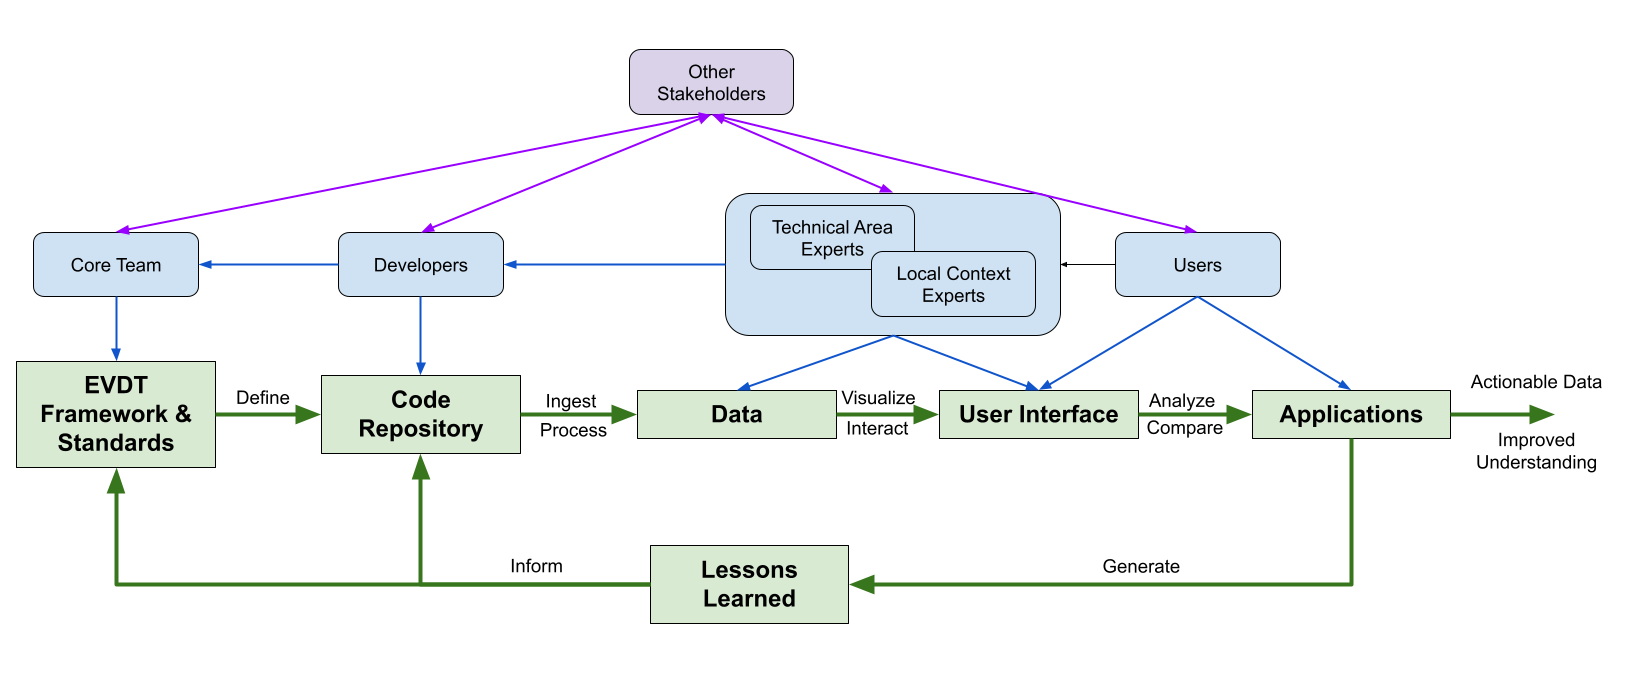
\includegraphics[scale=0.25]{Figures/chap3/Graphic_2_Development.png}
	\caption[The EVDT development pipeline] {The EVDT development pipeline. Note that the different community groups, shown in blue, are not necessarily discrete and one individual could simultaneously participate in multiple.}
	\label{fig:development}
\end{figure}

Some of the categories of \ac{evdt} community members shown in the blue boxes of Figure \ref{fig:development} require further explanation. What follows will be a generalized discussion of these categories. Specific instances for this thesis are discussed in Chapters \ref{ch:mangroves} and \ref{ch:vida}.

Moving from left to right, the \textit{Core Team} refers to those directly involved in the development of the \ac{evdt} Framework. Right now this is essentially a set of researchers in Space Enabled and some close academic affiliates. This team is likely to remain predominently academic moving forward, though could transition to involving individuals or organizations from \acp{ngo} in the future. The members of this team will typically have expertise with sustainable development and \acp{dss}, significant experience with \ac{evdt}, and investment in its success. Particularly once \ac{evdt} is more developed, this core team is likely to be formally defined.

The \textit{Developers} includes all those who actively develop the models, user interfaces, visualizations, and other associated aspects of the \ac{dss} software for the various \ac{evdt} projects. These will typically be individuals with expertise in \ac{gis}, coding, and/or data processing. Thus they are likely to work in academia or as analysts in a government agency or \ac{ngo}, though the project will be open source, membership in this category will not be formally defined and participation will be encouraged at any level of expertise or degree of involvement. Currently the Developer team is largely the same as the Core Team, though we have some developer involvement from other collaborators as well.

\textit{Technical Area Experts} refers to experts in some relevant domain to an \ac{evdt} project but are consulted but not directly involved in the ongoing development of the \ac{evdt} Framework and code repository. This could include individuals such as ecosystem services economists, human mobility researchers, or fisheries experts. They will typically come from the ranks of academia, though it is not unreasonable to expect some number of government analysts or \ac{ngo} researchers. As discussed in Chapter \ref{ch:theory}, sustainable development is made up of multiple domains interacting in a complex \ac{sets}. Each of these domains (including the \ac{evdt} domains) have their own disciplinary history and reservoir of technical expertise. While we cannot rely upon them to make all of society's decisions, we can and should rely upon their particular expert advice. 

\textit{Local Context Experts} refers to those who have a high level of knowledge of the \ac{sets} and stakeholders of a particular \ac{evdt} project. This could include a local community leader, an experienced activist, or a local government official. This category is grouped together with \textit{Technical Area Experts} as the line between the two is oftentimes blurry. A local university researcher who studies the economics of informal housing and who specializes in the city involved with a particular \ac{evdt} project is arguably both a Technical Area Expert and a Local Context Expert. The importance of the complementary effect of having both kinds of experts is attested to throughout the literature, including in \textit{Data Action} \cite{williamsDataActionUsing2020} and \textit{Data Science in Context} \cite{spectorDataScienceContext2022}. 

\textit{Users} refers to those who directly use the \ac{dss} software developed through an \ac{evdt} project. Exactly who these are will depend on the specific project and thus their level of experience with mapping, earth science, or development may vary significantly. They should be direct stakeholders in the specific \ac{evdt} project and have some involvement with the decision-making process (though not necessarily formal involvement). 

It should also be emphasized that while Figure \ref{fig:development} is fairly linear, the \ac{evdt} Framework emphasizes collaborative development. One person may serve multiple roles in the pipeline and, even if not, stakeholders, including users, should be involved throughout the \ac{dss} development process.

As the number of applications increase and the code is refined, the various models used in the applications may themselves be the first members of an openly accessible library of models. Potential user groups could adapt and reuse \ac{evdt} components in other applications, without having to start from scratch. Initially this would likely still require significant code expertise, but it is entirely possible for functionality to be created to allow for `plug-and-play.' A user may be able to, in browser or on desktop, select a geographic area of interest (e.g. the Sóc Trăng Province of Vietnam), select an environmental model (e.g. coastal forest health), a societal impact model (e.g. cyclone vulnerability), a decision-making model (land use conversion and conservation policy), and a technology model (satellite versus in-situ monitoring), all without writing a line of code (though perhaps being required to import new datasets themselves). Such functionality, along with the recruitment pipeline shown in Figure \ref{fig:development}, help to expand participation in all aspects of \ac{evdt}. In this way the user base will be expanded beyond initially invested experts.

We are cognizant that making \ac{evdt} truly participatory is easier said than done, but we do believe it is a worthy goal. In addition to model interoperability standardization, the code moderators will need to specify accessibility norms as well, so as to ensure usability by individuals with a wide range of backgrounds. Existing prototypes have made some steps in this direction, by having multiple language options available. Thus far, this has been accomplished by existing language knowledge of code moderators as well as the occasional volunteer translator, but some more targeted efforts may be required in the future to specifically recruit translators for targeted languages.

Language is not the only accessibility barrier, however. Terminology, presentation, and interactiveness can also be differentiately accessible to different individuals, depending factors such as educational or cultural background. That said, these difficulties can be addressed via some of the same methods that are already core to the \ac{evdt} methodology: namely partnerships with local collaborators; stakeholder analysis; and iterative, participative design. 

Another consideration in the future of \ac{evdt} are the types of applications that it will be used for. Some potential applications include:

\begin{enumerate} \setlength{\itemsep}{0pt} \setlength{\parskip}{0pt}
    \item To inform sustainable development policies. Ex) Comparing the impact of different conservation and zoning policies on the local environment and on economic outcomes.  \label{item:policy}
    \item To educate on the connections between the different \ac{evdt} domains. Ex) Demonstrating the local ecosystem services value of treecover in an urban environment.
	\item To facilitate the comparison of different remote sensing data products for particular applications. Ex) Considering whether to commission periodic aerial surveys of an area or to rely on "free" civil satellite data, such as Landsat and Sentinel. \label{item:data}.
    \item To facilitate the exploration and evaluation of new sensing technology architectures for particular applications. Ex) Designing a new \ac{lidar} satellite to assist forest management in a particular region. \label{item:tech}
    \item To facilitate scientific research on ecosystem services and/or the impacts of human behavior on the environment. Ex) Simulating different casual connections and comparing the simulated data with historical data, to assess the strength of those connections.
    \item To provide a basis for studies of the effectiveness of different \ac{dss} attributes. Ex) Assessing visualization techniques, workshop formats, etc. \label{item:user}
\end{enumerate}

These applications are varying levels of interest and importance to different stakeholders, and some could potentially be viewed as competing for development resources and focus. In some cases they may rely upon different configurations of the \ac{evdt} components, as shown in Figure \ref{fig:combo}. For instance Items \ref{item:data} and \ref{item:tech} (best served by configuration B of Figure \ref{fig:combo}) require a functional model of the relationships between different remote observation design parameters and performance parameters, along with a means of visualizing and exploring the tradespace (as has been proposed by Siddiqi et al. \cite{siddiqiValuingNewEarth2019}). A user who is predominantly interested in Item \ref{item:policy} (configuration A) may find this functionality irrelevant or outright distracting.

On the other hand, some applications are more complementary. While the Item \ref{item:policy} is likely to be a government official or community member while the Item \ref{item:user} user is likely to be an academic researcher, the findings from Item \ref{item:user} would result in the design of \ac{evdt} being improved, so as better serve the needs of the Item \ref{item:policy} user.

As explained in the introduction to Section \ref{sec:questions}, one of the goals of the \ac{evdt} Framework is to bring some of the benefits or \ac{eo} and environmental modeling to a smaller spatial scale. When operating on such scales, we must be careful about what metrics of human wellness we use. Historically social indicators tended to be defined for city, province, or national areas, the \acp{mdg} and \acp{sdg} being the preeminent examples of the latter. Advances in \ac{gis}, however did enable the creation of more neighborhood level indicators starting in the late 1990s \cite{sawickiNeighborhoodIndicatorsReview1996}. Sawicki and Flynn argue that one must specify the goals before specifying what indicators to use. From their list of possible aims, the following are the most relevant to \ac{evdt} \cite{sawickiNeighborhoodIndicatorsReview1996}:

\begin{itemize}[itemsep=0pt,parsep=0pt]
	\item{Developing dynamic models of neighborhood change}
	\item{Evaluating the likely impact of existing and/or proposed policies on neighborhoods and/or their residents.}
	\item{Measuring inequality over space and time both within and between regions.}
\end{itemize}

Ideally, \ac{evdt} would be open to all these applications and more. In practice, care must be taken so that interests of one user group do not unintentionally dominate those of others or, worse, that the interests of the developers do not send them on a path counter to the interests of the users. This will thus require ongoing discussion and consideration with the \ac{evdt} community.

It should also be recognized that not all users will engage with the \ac{evdt} \ac{dss} software products directly or in the same way. As shown in Figure \ref{fig:development}, some stakeholders and community members will participate in the \ac{saf} process, but may not directly interact with the \ac{evdt} software products themselves. This is both due to the fact that many people are unlikely to have the time or inclination to do so (understandably so) and due to various barriers that will doubtlessly remain despite the efforts of \ac{evdt} developers. Such barriers include access to the internet, computing power, and electricity. While all of these are becoming available to an increasing number of people globally, they are by no means ubiquitous. Initial prototypes have \ac{evdt} have pursued both offline, desktop version and online, browser-based versions to try and accomodate different levels of resource access. Such issues will need to be considered as part of future development decisions as well.

Finally, this envisioned development and expansion process is fundamentally a "snowball model." Existing team members collaborate with new partners and their communities. This results in additional team members who can then collaborate with others. \ac{evdt} may (and should aim) to one day be easily accessible even in the absence of connections to existing community members, but that is not in the immediate future.

\clearpage
\begin{figure}[!htb]
	\centering
	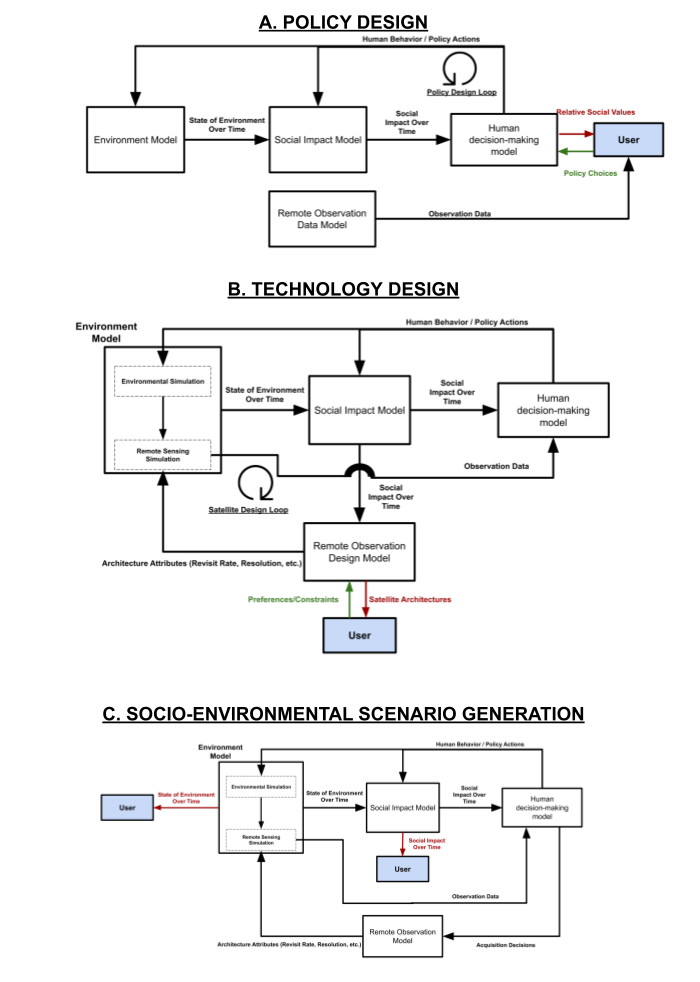
\includegraphics[scale=0.5]{Figures/chap3/Loops_Combined.png}
	\caption{Three example EVDT research configurations}
	\label{fig:combo}
\end{figure}
\clearpage







%%%%%%%%%%%%%%


%
%Position \ac{evdt} using the different dimensions of models proposed in \cite{harrisQuantitativeModelsUrban1972}:
%
%\begin{enumerate}[itemsep=0pt,parsep=0pt]
%	\item{descriptive vs. analytic}
%	\item{holistic vs. partial}
%	\item{macro vs. micro}
%	\item{static vs. dynamic}
%	\item{deterministic vs. probabilistic}
%	\item{simultaneous vs. sequential (directly calculate the output or go through intermediate phases)}
%\end{enumerate}


%Miller argues that, despite the historical dificulties that integrated urban models have had, there is reason to be optimistic about the state of the art moving forward, particularly for integrating transportation and land-use models in particular \cite{millerIntegratedUrbanModeling2018}. <---important to discuss at more length


\section{\hlc[green]{Conclusion}} \label{sec:evdt-conclusion}

This chapter laid out the \acf{evdt} Framework, providing detail on each of its five elements:

\begin{enumerate}[label=\emph{\Alph*},itemsep=0pt,parsep=0pt]
	\item{The use of systems architecture \& stakeholder analysis to identify needs, design the \ac{dss}, and understand the context through the use of the \acf{saf}. This requires significant engagement with as many of the stakeholders as is feasible (if not more). Usually two or more iterations through the \ac{saf} cycle are required.}
	\item{Collaborative development of the \ac{dss} that continues that stakeholder engagement.}
	\item{A concept of the sustainable development application as a complex \ac{sets}, typically involving the Environment, Human Vulnerability and Societal Impact, Human Behavior and Decision-Making, and Technology Design. This concept undergirds the \ac{dss} architecture and is critical as it provides the capability both for detailed technical analysis as well as feeding back into the design of data collection systems .}
	\item{An interactive \ac{dss}. This can take the form of an in-browser page, a standalone application for a computer or phone, or even a tabletop exercise with paper documents.}
	\item{A consideration towards modularity and re-use in future applications. This includes both technical components of the \ac{dss} product and broader capacity building in the community.}
\end{enumerate}

In doing so this chapter has provided Research Deliverable 1b:

\blockquote{\textit{A proposed framework for applying systems engineering for sustainable development in an participatory and social-justice-oriented manner.}}

While this chapter includes some brief mentions and anecdotes about concrete applications of the \ac{evdt} Framework, it still remains to actually see \ac{evdt} in action. Such applications is precisely what the following two chapters (Chapters \ref{ch:mangroves} and \ref{ch:vida}). The first is focused on mangrove conservation and economic development in a particular neighborhood of Rio de Janeiro, Brazil. The second is focused much more broadly on \ac{covid} response across a variety of metropolitan areas.

Another limitation of this chapter is that it primarily considered the \ac{evdt} Framework as a static, finished creation, sprung into existence fully formed like Athena. This, of course is an oversimplification. The \ac{evdt} Framework was created in an incremental, iterative, and syncretic fashion over the course of the past few years, from early conference presentations \cite{reidCombiningSocialEnvironmental2019} to this thesis. Similarly, the \ac{evdt} Framework is by no means final. The very case studies presented in the following chapters provided significant learning opportunities for future revision, as have projects undertaken by others such as Ovienmhada \cite{ovienmhadaEnvironmentVulnerabilityDecisionTechnologyModelingFramework2021, ovienmhadaEarthObservationTechnology2020} and Lombardo \cite{lombardoEnvironmentVulnerabilityDecisionTechnologyFrameworkDecision2022}. Chapter \ref{ch:conclusion} will review these lessons, including discussing how the case studies would have been performed differently in retrospect. It will also provide a potential road map for how the \ac{evdt} Framework may develop in the future.
